\chapter{Motion Segmentation Pipeline}
In this chapter we explain in detail the relevant stages of our motion segmentation pipeline. For this purpose we heavily rely on the definitions of \textit{Optical Flow} and \textit{Spectral Clustering} introduced in the previous chapter. We start by restating the initial problem statement our pipeline tries to solve. Moreover, for each stage, we describe its required input data and what output it generates. Lastly, we also mention all assumptions and induced limitations for each pipeline stage. \\ \\
The problem statement our pipeline solves is defined as follows: Given a sequence of frames that form a video and their associated depth maps. Then our goal is to segment the images into regions that mask regions of coherent and independent rigidly moving objects. Therefore we describe the implementation of a motion segmentation pipeline that addresses this problem statement by using optical flow fields. In addition, our implementation should be robust according to complex camera movement and noise, should be able to deal with occlusions and missing data, should be able to handle many moving objects, and lastly, it should be able to detect several fast moving rigid objects. \\ \\
The idea of such a segmentation is to identify and extract meaningful rigid motions from a steady background. The motion of an object in a video sequence can usually not be considered as independent in a per frame basis, since typical object motions proceed over a series of frame. From the previous chapter we know that using optical flow fields enables us to run a consistent tracking of feature points in a video. Hence, the optical flow is an ideal cue for making motion grouping decisions. In our case we use the flow fields to generate motion point trajectories.
\begin{figure}[H]
\begin{center}
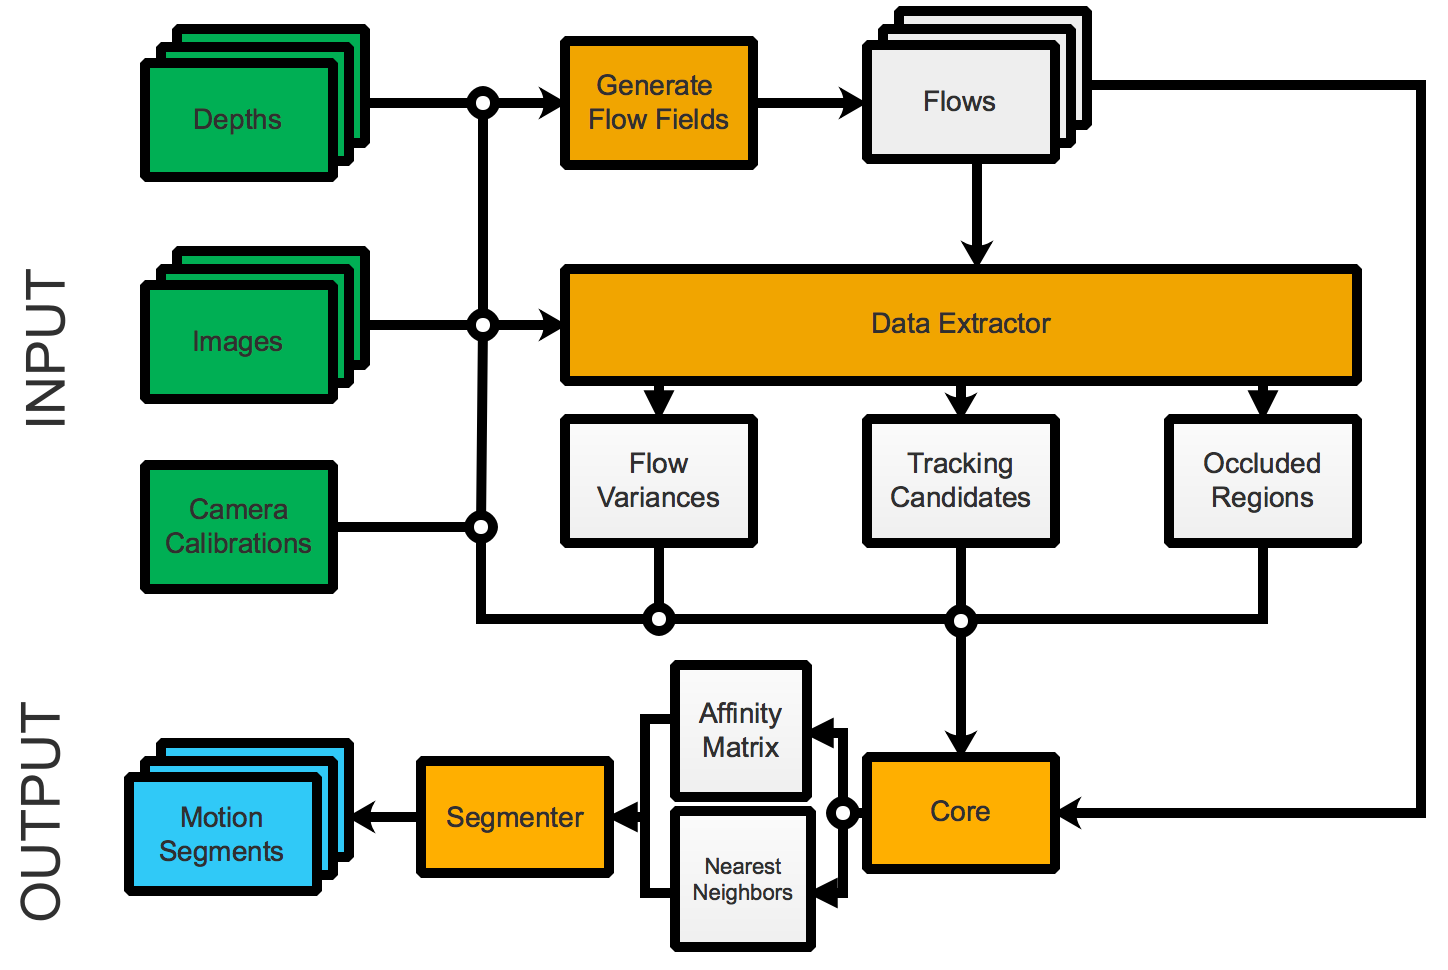
\includegraphics[width=0.9\linewidth] {implementation/pipeline}
\end{center}
\caption[Motion Segmentation Pipeline]{A schematic illustration of the structure of our pipeline. Individual pipeline components are drawn as orange boxes. The initial inputs are drawn as green boxes, the resulting final output as a blue box. Intermediate outputs are drawn as gray boxes. The arrows indicate the data-flow, whereas the white dots indicate a data-flow multiplexing. That means that data, which flow fields through such a dot is used by several pipeline components.}
\label{fig:pipeline_schematic}
\end{figure}
In the following let us briefly outline the main stages of our motion segmentation pipeline, which is visualized in Figure $\ref{fig:pipeline_schematic}$:
\begin{enumerate}
\item \textbf{Dataset Preparations} (Sec. $\ref{sec:dataset_preparations}$): Initially, the frames and depth maps of a given RGB-D video have to be extracted and named according to our pipeline naming conventions. Moreover, the depth map range is normalized in meter units.
\item \textbf{Generate Optical Flow Fields} (Sec. $\ref{sec:generate_of}$): In this stage the forward- and backward-flow fields are computed on the input sequence.
\item \textbf{Data Extractor} (Sec. $\ref{sec:data_extraction}$): In this stage we extract traceable feature locations in our images. In addition, a mask containing all invalid tracking locations per image is computed by checking whether the forward and backward flow correspond to each other. Optionally depth data, flow and depth variances and color maps are extracted that are used at within a later pipeline stage. 
\item \textbf{Trajectory Tracking} (Sec. $\ref{sec:trajectory_tracking}$): The previously computed flow fields are used to perform a point tracking on the extracted traceable features. The ordered sequence of tracking points of a feature is called trajectory.
\item \textbf{Affinity Matrix Generation} (Sec. $\ref{sec:affinity_matrix_impl}$): In this stage the similarities between all trajectory pairs are computed. This is achieved by computing the color-, spatial- and motion distance between the overlapping segments of a pair and combining them in a certain way.
\item \textbf{Segmenter}: Our pipeline offers two types of segmentations: sparse and dense. 
	\begin{enumerate}
	\item \textbf{Sparse Motion Segmentation} (Sec. $\ref{sec:sparse_motion_segmentation}$): Using the affinity matrix plus the nearest neighbouring trajectories per trajectory, we can compute its sparse segmentation by either applying a spectral clustering on the affinity matrix or by reformulating the problem as a graph cut problem. 
	\item \textbf{Dense Segmentation} (Sec. $\ref{sec:dense_motion_segmentation}$): Optionally, our pipeline allows us to transform the sparse segmentation into a dense segmentation. 	
	\end{enumerate}
\end{enumerate}
In the following sections we examine and discuss each individual pipeline stage in detail. 

\section{Dataset Preparations}
\label{sec:dataset_preparations}
The preparation of input datasets is the very first stage of our pipeline. Initially, we have to either capture a video using one of our capturing devices or use an existing video sequence. Next, we extract all the frames from the considered video. In case there are also depth maps$\footnote{In case we are working with depth data, we assume that there exists one depth map per frame. Our pipeline assumes, that the values in the depth images are in meter units}$ available, they are transformed in such a way that their value range is in meter units. An example of a color frame and its depth field is shown in Figure $\ref{fig:color_and_depth_image}$.
\begin{figure}[H]
\begin{center}
\subfigure[Color Frame]{
   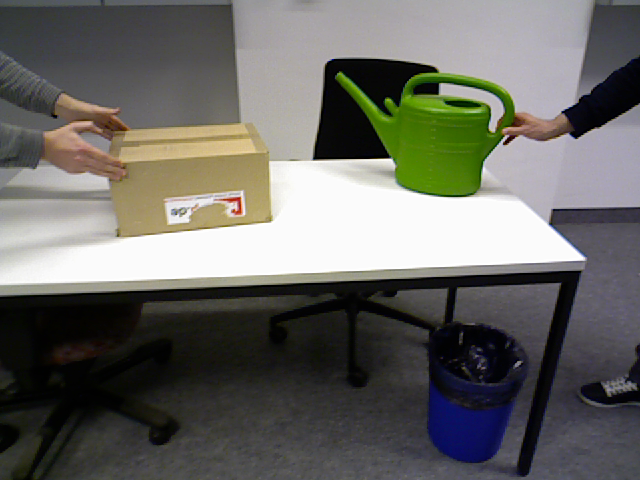
\includegraphics[width=0.48\linewidth] {implementation/preproc/18}
   \label{fig:color_and_depth_image_a}
}
\subfigure[Depth Field]{
   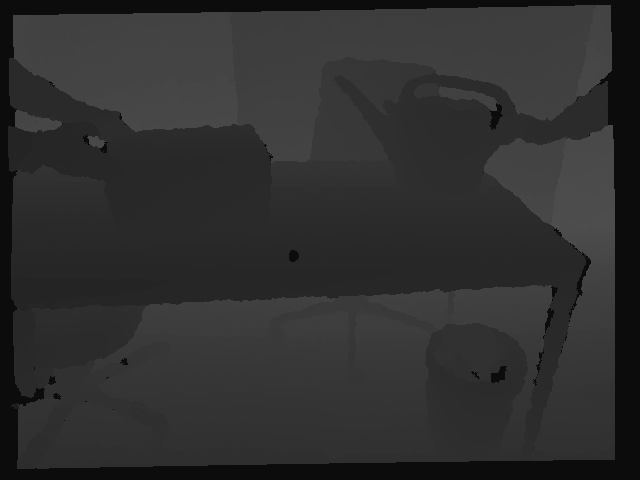
\includegraphics[width=0.48\linewidth] {implementation/preproc/depth_18}
   \label{fig:color_and_depth_image_b}
}
\end{center}
\caption[Color and Depth Image]{Visualizing a color frame and a depth field of the \textit{Bonn Water Can} dataset$\footnotemark$.}
\label{fig:color_and_depth_image}
\end{figure}
\footnotetext{Source of the images shown in Figure \ref{fig:color_and_depth_image}: \url{http://www.ais.uni-bonn.de/download/rigidmultibody/}}
Our pipeline assumes a well-enumeration of its video frames, meaning that the image, which corresponds to the $k-th$ frame is referenced by the name \textit{k}. Moreover depth fields follow the same naming convention and thus are similarly named as its corresponding video frame. A listing of our datasets can be found in Section~\ref{sec:datasets} on page~\pageref{sec:datasets}.

\section{Generate Optical Flow Fields}
\label{sec:generate_of}
In our pipeline we rely heavily on optical flow fields. In particular, flow fields are used to perform the point tracking required to extract motion trajectories, to detect occlusions and to compute affinities between trajectories. Therefore, the quality of the flow fields highly affects the final outcome of the motion segmentation. \\ \\
A conceptual idea as well as a mathematical formulation of optical flow fields is provided in Section $\ref{sec:optical_flow}$ on page $\pageref{sec:optical_flow}$. However, in principle, the optical flow represents a displacement field that defines where a certain point in a frame is mapped to in its successive frame. \\ \\
In this stage we want to generate the following optical flow fields on the frames of a given dataset video:
\begin{itemize}
	\item The \textbf{forward flow} fields: Refers to the optical flow between a frame and its successor frame.
	\item The \textbf{backward flow} fields: Refers to the optical flow between a frame and its predecessor frame.
\end{itemize}
For the actual computation of the flow fields we rely on existing implementations. In particular we use the freely available implementations of the methods discussed in Section $\ref{sec:optical_flow}$ on page $\pageref{sec:optical_flow}$. In the following is a short list of the flow fields integrated in our pipelines and their main properties:
\begin{itemize}
\item The enhanced version of the original flow method proposed by Horn and Schunck (\textbf{HS}): This flow estimation method is a tweaked version of H.S. original formulation. The authors offer a freely available Matlab implementation that has a decent run-time. Please note that this implementation does not make use of depth maps to compute the flow estimations.
	\begin{itemize}
	\item Simple formulation and fast to run.
	\item Matlab implementation freely available.
	\item Does not make use of depth fields.
	\end{itemize}
\item The large displacement optical flow estimation (\textbf{LDOF}): LDOF implements a flow estimation method that is capable of handling large motions and thus yields a better quality fast moving objects flow estimations. This method, however, does also not make use of depth fields. The authors offer a freely available, compiled C++ program. The program has an intermediate runtime of about 30 seconds per $480 \times 640$ pixel frame.
	\begin{itemize}
	\item Can handle large displacements, i.e. fast moving objects.
	\item Compiled C program freely available
	\item Does not make use of depth fields
	\end{itemize}
\item The Semi-rigid scene flow (\textbf{SRSF}) method: The authors offer a partially available code basis that can be compiled to a executable program. The program can only generate motion segmentations for datasets that have an image resolution of $480 \times 640$ pixels. Since the program makes use of depth fields, corresponding depth maps have to be provided in the pipeline's formatting conventions. A detailed descriptions about their pipeline conventions can be found in their documentation$\footnote{See \url{http://lmb.informatik.uni-freiburg.de/Publications/2014/Bro14/}}$. 
	\begin{itemize}
	\item Makes use of depth maps: formulates a local and global motion by jointly using intensity and depth data.
	\item Models motion as a global rigid motion plus a non-rigid residual
	\item Free C++ code available, some parts are only available as binaries.
	\item Can only be run on videos with a resolution of $640 \times 480$ pixels
	\end{itemize}	
\item The Layered RGBD flow (\textbf{LRGBD}) method: The LRGBD method segments motion into layers ordered according to the depth ranking. The authors offer a freely available Matlab implementation.
	\begin{itemize}
	\item Makes use of depths to handle occlusions
	\item Layered RGBD scene flow estimation method
	\item Very slow in terms of computation time
	\item They offer a freely available Matlab implementation
	\end{itemize}
\end{itemize}
For this thesis let us use the abbreviations defined in the list above when referring to a particular flow method. To conclude this section we demonstrate in Figure $\ref{fig:flow_method_flows}$ an example output produced by running these methods on a common frame:
\begin{figure}[H]
\begin{center}
\subfigure[Color Frame]{
   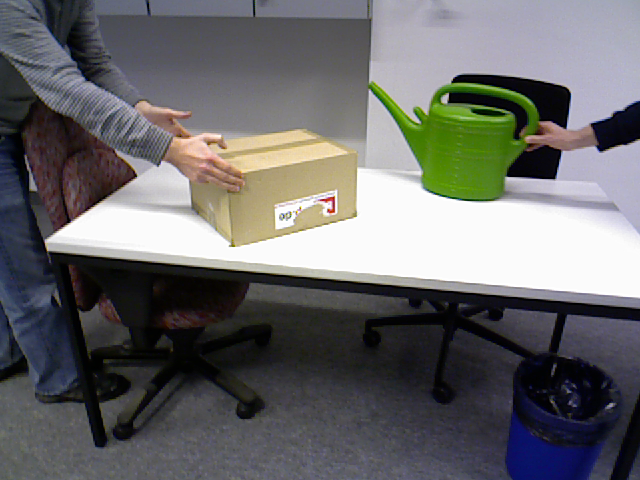
\includegraphics[width=0.47\linewidth] {implementation/flow_methods/f30}
   \label{fig:flow_method_flows_a}
}
\subfigure[Depth Field]{
   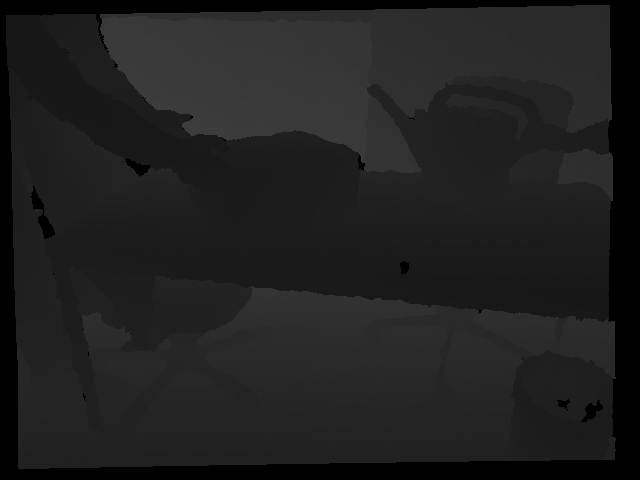
\includegraphics[width=0.47\linewidth] {implementation/flow_methods/d30}
   \label{fig:flow_method_flows_b}
}
~
\subfigure[HS]{
   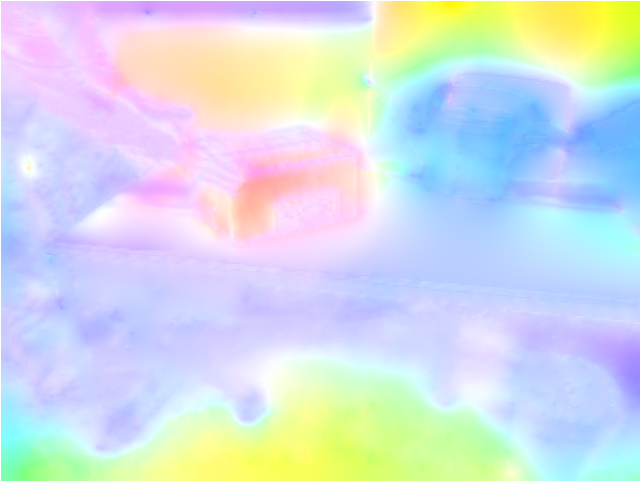
\includegraphics[width=0.47\linewidth] {implementation/flow_methods/hs}
   \label{fig:flow_method_flows_a}
}
\subfigure[LDOF]{
   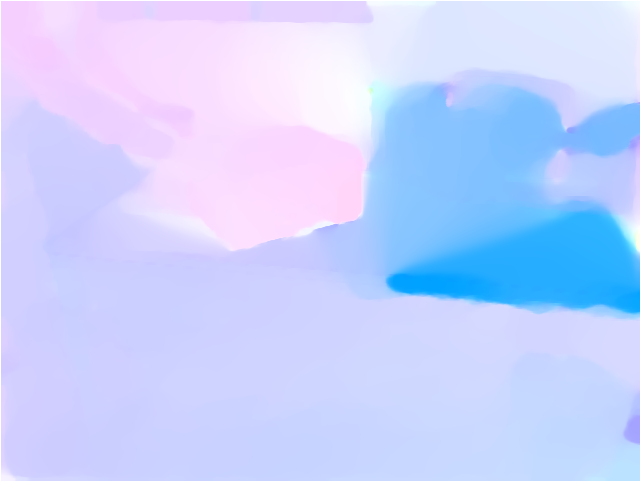
\includegraphics[width=0.47\linewidth] {implementation/flow_methods/ldof}
   \label{fig:flow_method_flows_b}
}
~
\subfigure[LRGBD]{
   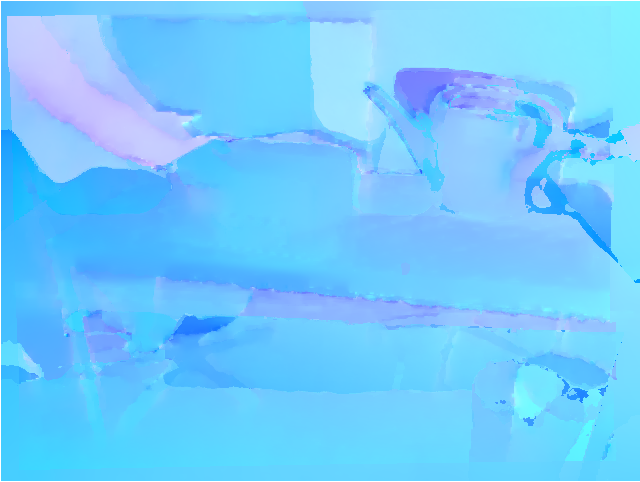
\includegraphics[width=0.47\linewidth] {implementation/flow_methods/lrgbd}
   \label{fig:flow_method_flows_c}
}
\subfigure[SRSF]{
   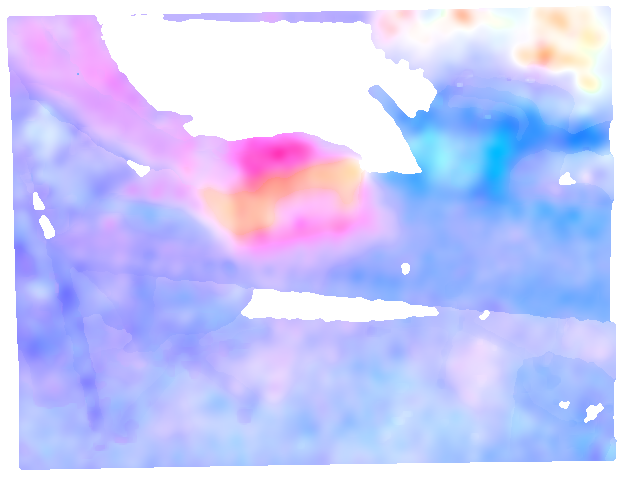
\includegraphics[width=0.47\linewidth] {implementation/flow_methods/srsf}
   \label{fig:flow_method_flows_d}
}
\end{center}
\caption[Flow Fields]{A visualization of the flow fields produced by our used flow methods when running them on frame 30 of \textit{Bonn Watercan} dataset$\footnotemark$. Please notice that the color encoding is the same as introduced in Section $\ref{sec:optical_flow}$ on page $\pageref{sec:optical_flow}$.}
\label{fig:flow_method_flows}
\end{figure}
\footnotetext{Source of the images shown in Figure \ref{fig:flow_method_flows}: \url{http://www.ais.uni-bonn.de/download/rigidmultibody/}}

\section{Data Extraction}
\label{sec:data_extraction}
In this section we offer the reader a detailed description of what data and how it is extracted. This pipeline stage can be understood as a pre-processing stage. \\ \\
In particular we will explain how meaningful image locations of moving objects are determined, how we detect occlusions and lastly how we normalize our flow fields to dump their estimation errors. Algorithm $\ref{alg:data_extraction}$ gives an overview of the involved steps in this stage.
\begin{algorithm}[H]
\caption{Data Extraction}
\begin{table}[H]
  \begin{tabular}{@{}lll@{}}
    \textbf{Input:} & Dataset Images \bf{F} \\
		& Forward- and Backward Optical Flow Fields \bf{OF} \\
 		& Depth Images (\emph{optional}) \bf{DI} \\
    \textbf{Output:} & Traceable Feature Locations \bf{TF} \\
    & Occluded Location Masks \bf{OM}\\
    & Cielab Color Images \bf{CI} \\
    & Flow Variances \bf{FV} \\
    & Depth Variances \bf{DV} \\
    
  \end{tabular} 
\end{table}
\setlength{\fboxrule}{0pt} 
\begin{boxedminipage}{1.0\textwidth}
  \begin{algorithmic}[1]
      \ForAll{$\text{frame } f \in \bf{F}$}
        \State $\text{Run Thresholded Harris Corner Detector}.$
		\State $\text{Append Sampled Features to } \bf{TF}.$
		\State $\text{Fetch } fwf,bwf \in \bf{OF} \text{ that belongs to f}.$
		\State $\text{Apply forward-backward-flow check on fwf and bwf} \bf{TF}.$
		\State $\text{Append invalid check locations to } \bf{OM}.$
		\State $\text{Apply a special variant of the bilateral filter on fwf}.$
		\State $\text{Append filtered flow to } \bf{FV}.$
		\State $\text{Transform f to CIE Lab Colorspace and append it to } \bf{CI}.$
		\State $\text{Fetch } df \in \bf{DI} \text{ that belongs to f}.$
		\State $\text{Apply a 2-pass special variant of the bilateral filter on } df$
		\State $\text{Append the filtered depth to } \bf{DV}$
      \EndFor
  \end{algorithmic}
  \end{boxedminipage}
  \vskip1.5pt
\label{alg:data_extraction}
\end{algorithm}
For every dataset frame we extract potential tracking candidates, the forward-and backward flow to the next frame, the occlusion map and colors in the CIE lab space, the normalized depth fields ranging in meter units and the depth-and flow variances. All this data is then saved to an individual file and used in a later pipeline stage.
\subsection{Tracking Candidates}
\label{sec:tracking_candidates}
Our implementation determines moving object regions by performing a grouping on motion trajectories. However, to form such trajectories we need to run a tracing on reliable motion features over the given video sequence. So, what are these features and how are they detected? \\ \\
In this section we therefore explain our approach on how to determine reliable and meaningful image locations that exhibit motion information and thus are suitable candidates to track. The found tracking candidates are later used as the starting position to trace features. Therefore, the quality of the candidates affects the detection of the moving objects. \\ \\
The simplest idea would be to simply track every pixel location. On one hand, this would indeed capture every moving object. On the other hand, however, this also would make the later involved motion segmentation task highly inefficient, yet infeasible for common image resolutions, because there would be simply too many trajectories to cluster. Therefore, we want a method which offers us a sparse sampling of the image locations and at the same time hits enough meaningful candidates. \\ \\
Ideally, we want to use a feature detector that ignores points in homogeneous areas$\footnote{Within a homogeneous area all flow vectors should look the same. However, due to errors present in the flow estimates, vectors in such regions can be perturbed. This might cause to produce incorrect segmentations, because such regions introduce new motion boundaries and thus negatively influence the segmentation.}$ but selects points that show structural information in their vicinity. Since image corners exhibit a lot of structural information a Harris detector, as described in Section $\ref{sec:harris_corner_detector}$), is a solid choice to approach this task. \\ \\
The idea of this detector is the following: A corner defines an intersection of two edges. Therefore, it represents a point in which the directions of these two edges change. For images this means that the gradient has a large variance at that location. \\ \\
It is possible to describe the average intensity change in any direction $(x,y)$
as a bilinear from
\begin{equation}
\left( x,y \right) M \colvec{x}{y}	
\end{equation}
Within the Harris detector code, every image location is then described in terms of the eigenvalues of $M$. Moreover, the detector uses the pixel-wise eigenvectors to measure the corner response. Good corners have a large intensity change in all directions and thus their measured response should be large and positive. A detailed formulation of the Harris corner detector can be found in Section $\ref{sec:harris_corner_detector}$ on page $\pageref{sec:harris_corner_detector}$. \\ \\
We apply the described Harris corner detector on every dataset image. This procedure yields a sparse set of traceable corner candidates per frame. Additionally, candidates with a too weak corner response are filtered according to a certain threshold value. This ensures that only strong edges and reliable features are being tracked. \\ \\
Lastly, for efficiency reasons, we spatially subsample the extracted locations. The subsampling is performed by applying a boolean grid with a specific cell size on the candidates, which acts as a selection mask to make subsequent pipeline steps tractable. This reduces the number of tracking candidates drastically and makes the sampling even more sparse. Hence, we have to track fewer features and the overall runtime decreases. \\ \\
The image locations of the remaining candidates are then dumped into a file. An example of this tracking candidate extraction procedure is illustrated in Figure $\ref{fig:tracable_candidates}$. \\ \\
\begin{figure}[H]
\begin{center}
\subfigure[Input Image]{
   \includegraphics[width=0.48\linewidth] {implementation/candidates/01}
   \label{fig:c14_f1_cand}
}
\subfigure[Sparse Candidates]{
   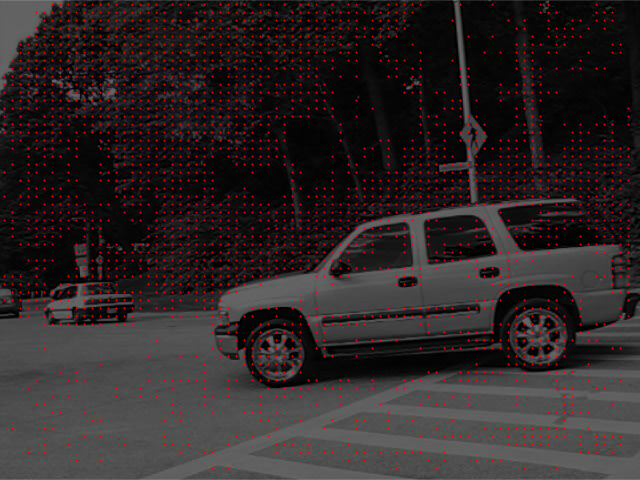
\includegraphics[width=0.48\linewidth] {implementation/candidates/candidates_sparse}
   \label{fig:c14_cand_sparse}
}
~
\subfigure[Harris Corners]{
   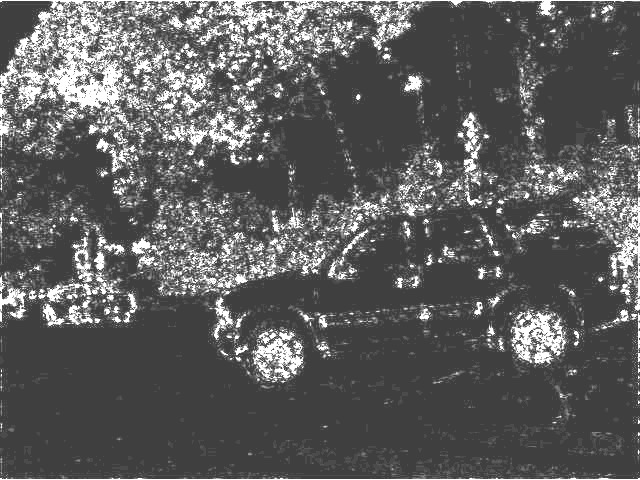
\includegraphics[width=0.48\linewidth] {implementation/candidates/out_corners}
   \label{fig:c14_cand_corners}
}
\subfigure[Dense Candidates]{
   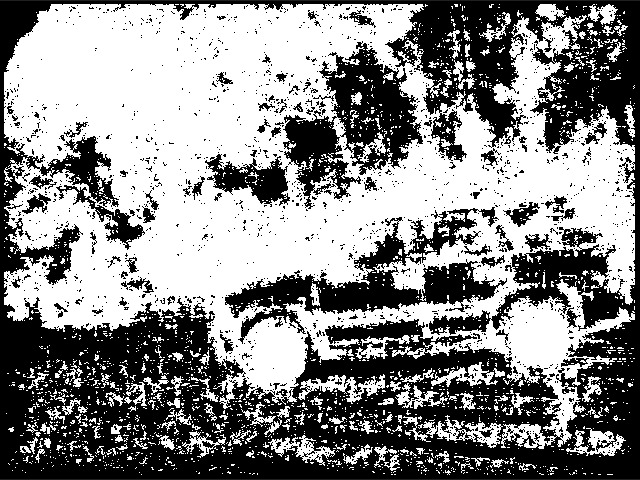
\includegraphics[width=0.48\linewidth] {implementation/candidates/c14_f1_candidates}
   \label{fig:c14_cand_dense}
}
\end{center}
\caption[Tracking Candidates]{A visualization of the tracking candidates' extraction stages. For a given input image as shown in Subfigure $\ref{fig:c14_f1_cand}$$\footnotemark$ we want to compute a sparse set of traceable feature locations as shown in Subfigure $\ref{fig:c14_cand_sparse}$. The candidates are visualized as a boolean matrix for which true means a valid traceable candidate and false an invalid tracking location.}
\label{fig:tracable_candidates}
\end{figure}
\footnotetext{Source of the image in Figure \ref{fig:c14_f1_cand}: the BMS-26 dataset from\\ 
\url{http://lmb.informatik.uni-freiburg.de/resources/datasets/}}
For any given dataset frame (Fig. $\ref{fig:c14_f1_cand}$) we compute its corners (Fig. $\ref{fig:c14_cand_sparse}$) by applying a Harris corner detector. By thresholding the resulting corners we reject too week candidates and thus obtain a dense sampling of candidate locations (Fig. $\ref{fig:c14_cand_dense}$). Lastly, by subsampling the candidates, we can further reduce their number and obtain the final sparse list of candidates (Fig. $\ref{fig:c14_cand_sparse}$). \\ \\ 
So, the remaining question is: How densely should we generate the sparse set of tracking candidates, i.e. what grid size should we select for our selection mask? \\ \\
In general it is always a trade-off between complexity and resolution. On one hand the optical flow is very redundant and typically bad at high frequency variations. On the other hand, choosing a too sparse sampling could result in missing important motion location such as small objects that are moving far away. To answer this question we ran different sampling rates on the tracking candidates and evaluated which size was able to produce the best motion segmentations. A visualization of tracking candidates produced by using different sampling rates is shown in Figure $\ref{fig:sampling_rate_candidates}$. 
\begin{figure}[H]
\begin{center}
\subfigure[Extreme Oversampling]{
   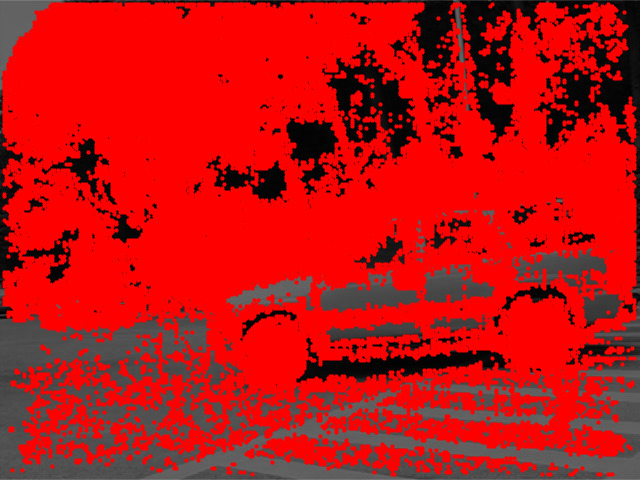
\includegraphics[width=0.48\linewidth] {implementation/candidates/sr_2}
   \label{fig:c14_extreme_oversampling}
}
\subfigure[Oversampling]{
   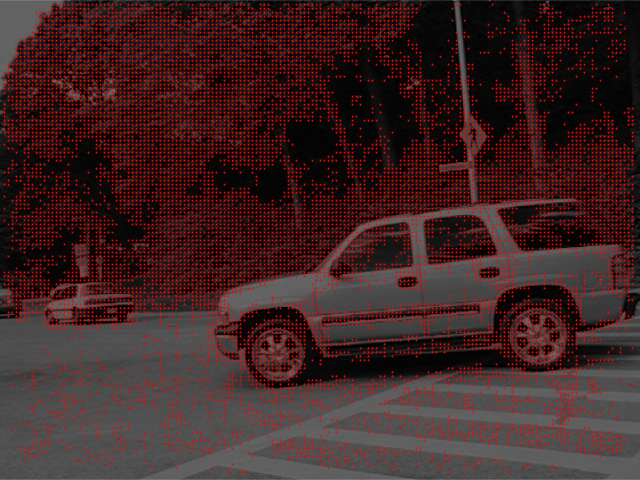
\includegraphics[width=0.48\linewidth] {implementation/candidates/sr_4}
   \label{fig:c14_oversampling}
}
~
\subfigure[Ideal Sampling Rate]{
   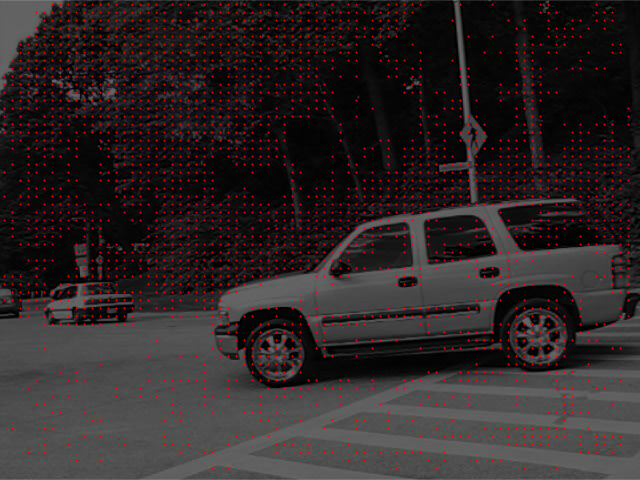
\includegraphics[width=0.48\linewidth] {implementation/candidates/sr_8}
   \label{fig:c14_ideal_sampling}
}
\subfigure[Undersampling]{
   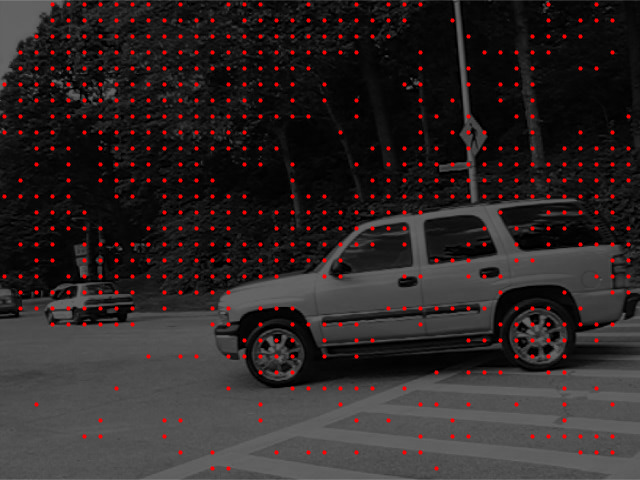
\includegraphics[width=0.48\linewidth] {implementation/candidates/sr_16}
   \label{fig:c14_undersampling}
}
\end{center}
\caption[Density Of Candidates For Different Sampling Rates]{A visualization$\footnotemark$ of different sampling rates of tracking candidates}
\label{fig:sampling_rate_candidates}
\end{figure}
\footnotetext{To generate the images in Figure \ref{fig:sampling_rate_candidates} I used the Cars dataset from the BMS-26 dataset: Source\\ 
\url{http://lmb.informatik.uni-freiburg.de/resources/datasets/}}
After tinkering with this parameter during our experiments we observed, that setting the cell size larger than 12 pixels causes a loss of details since there are not enough points to cover small object parts. Also, we observe that cells smaller than 6 pixels waste computation time as smaller objects tend to get smoothed away. Hence, our pipeline samples every 8th pixel by default. However, note that it is still possible to manually assign a different value to this parameter. \\ \\
Finally, there is one optional post-processing stage, which removes all candidates that map to a too weak optical flow vector. This reduction is implemented as following: We use the tracking candidate of a frame as lookup coordinates$\footnote{Sine these points are real valued but lookup indices are supposed to be integer values, we perform a bilinear interpolation on the discrete flow field at the given lookup coordinate.}$ in their corresponding forward flow fields and compute their magnitude. Then, every candidate that maps to a magnitude value smaller than the largest 10 percent of the determined flow magnitudes is discarded. We repeat this procedure for every frame. Doing so drastically reduces the total number of candidates. However this procedure may also cancel out useful motion locations. Nevertheless, most of the time this post-processing only removes candidates that belong to the background$\footnote{By \textit{background} we refer to pixel locations that do not map to a moving object.}$. Additionally, Figure $\ref{fig:tracable_candidates_strict}$ graphically illustrates the idea behind this filtering approach.
\begin{figure}[H]
\begin{center}
\subfigure[Subselection of all Dense Candidates]{
   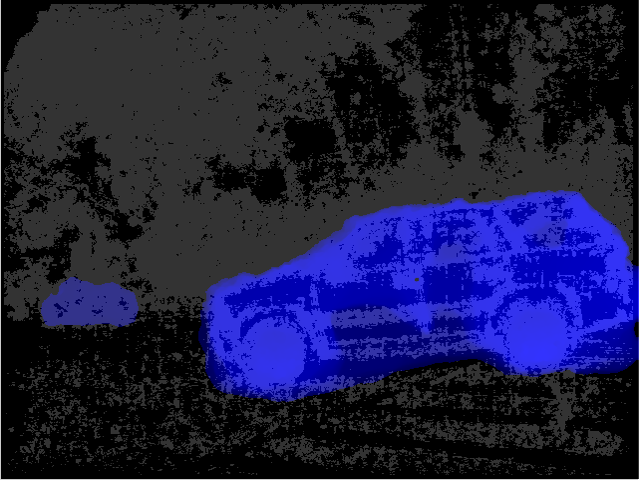
\includegraphics[width=0.48\linewidth] {implementation/candidates/subsel_flow_mags}
   \label{fig:c14_f1_cand_dense_2}
}
\subfigure[Strict Dense Candidates]{
   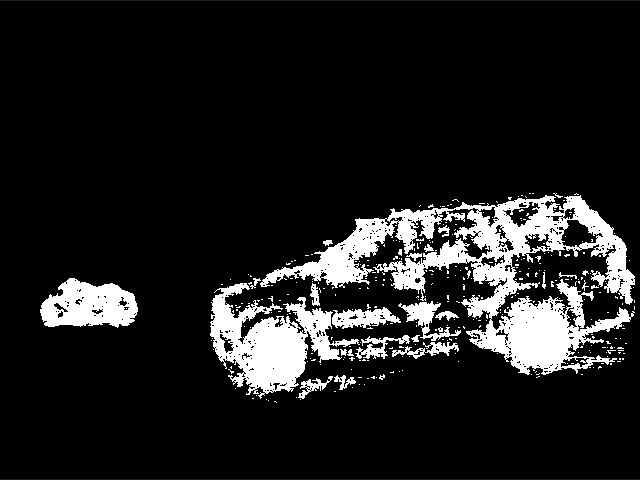
\includegraphics[width=0.48\linewidth] {implementation/candidates/strict_dense_candidates}
   \label{fig:c14_cand_dense_strict}
}
\end{center}
\caption[Strict Dense Candidates]{A visualization$\footnotemark$ of the post-processed traceable candidate locations. On the left side, all extracted candidate locations overlaid by the flow magnitudes (in blue), on the right, an image of the reduced candidates.}
\label{fig:tracable_candidates_strict}
\end{figure}
\footnotetext{To generate the images in Figure \ref{fig:tracable_candidates_strict} I used the Cars dataset from the BMS-26 dataset: Source\\ 
\url{http://lmb.informatik.uni-freiburg.de/resources/datasets/}}
In the image on the left (Fig. $\ref{fig:tracable_candidates_strict}$) we see the set of all dense tracking candidates overlaid by their flow magnitudes (the bluish masks). The stronger the magnitude, the more bluish the mask is colored. We make the trivial observation that the moving objects themselves correspond to the top flow magnitudes. Hence, filtering the tracking candidates by their flow magnitudes yields only tracking candidates located at moving objects (Fig. $\ref{fig:c14_cand_dense_strict}$). \\ \\
Both moving objects in the shown example are preserved and only background pixels are removed. However, keep in mind that this post-processing may filter small, meaningful motions. Especially, when there is a lot of camera motion involved, this approach may fail. \\ \\
Up to this moment we know \textit{when} (i.e. in what frame) and \textit{where} (i.e. at which location) we have to \textit{start} trajectories while running our point tracker. Moreover, by using the forward flow fields we know where the extracted features have to be tracked to in their successive frame. However, what we still do not know is \textit{when to end} the tracking of a trajectory. Usually, a trajectory is supposed to end when it gets occluded by an obstacle. In the next section we discus how to find such occluded regions.

\subsection{Occlusion Detection}
\label{sec:occlusion_det}
In this section we discuss a technique, which allows us to determine when to stop tracking a trajectory. This is particularly important since without stopping the tracking process within occluded regions, two distinct objects would be tracked by the same trajectory. In such a case groupings on motion trajectories would be very erroneous and thus would negatively affect the motion segmentation quality. \\ \\
The previously determined tracking candidates are used as starting points for point tracking. For every tracking candidate we determine its \textit{tracked to} position by adding the appropriate forward flow. However, this approach is very prone to create errors due to the use of incorrect flow estimations or the presence of occluded regions. \\ \\
Occlusion may occur whenever a previously visible object gets covered by another object. For instance, when an object close to the camera gets directly in front of an object in the background. Continuing to trace a point in an occluded region yields an incorrect tracking, because two distinct objects are tracked by the same trajectory. Thus, we have to stop tracking points as soon as they get occluded.
\begin{figure}[H]
\begin{center}
\subfigure[Input Image]{
   \includegraphics[width=0.48\linewidth] {implementation/occlusion/01}
   \label{fig:c14_f1_occ}
}
\subfigure[Occluded Regions]{
   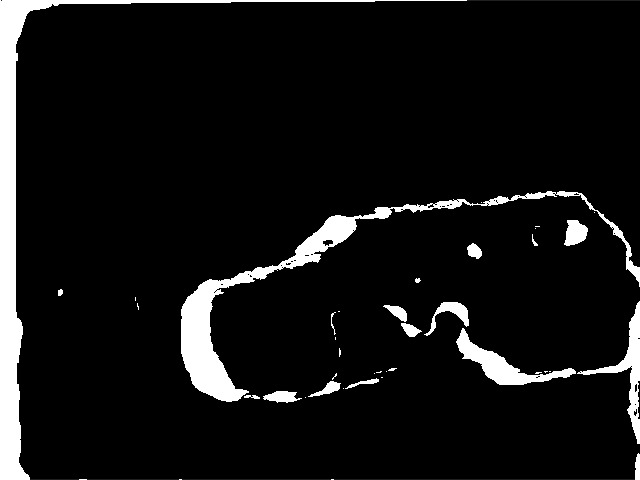
\includegraphics[width=0.48\linewidth] {implementation/occlusion/invalid_regsions}
   \label{fig:c14_invalid_regions}
}
\end{center}
\caption[Occluded Regions]{A visualization of occluded regions. On the left, a color video frame$\footnotemark$ and on the right its corresponding occluded regions (white pixels).}
\label{fig:invalid_regions}
\end{figure}
\footnotetext{Source of the image in Figure \ref{fig:c14_f1_occ}: the BMS-26 dataset from\\ 
\url{http://lmb.informatik.uni-freiburg.de/resources/datasets/}}
In tracking tasks, occlusion is usually detected by comparing the appearance of the local neighborhood of the tracked point over time. However, following the ideas described in $\cite{Bro10c}$, we detect occlusions by verifying a consistency check between the forward- and backward flow fields. Such a verification is performed by applying the backward flow $\hat{w}_t$ to its continued tracked point $p_{t+1}$. Finally we have to check whether the resulting point has the same origin $\hat{p}_t$ as the actual tracked from position $p_t$. Additionally, we visually outlined this concept of occlusion detection in Figure $\ref{fig:occlusion_detection}$. Moreover, an example of occluded regions produced by following our approach is shown in Figure $\ref{fig:invalid_regions}$.
\begin{figure}[H]
\begin{center}
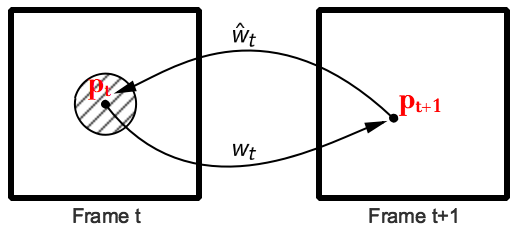
\includegraphics[width=0.6\linewidth] {implementation/occlusion/occ_det}
\end{center}
\caption[Occlusion Detection]{Conceptual illustration of occlusion detection. For any tracking candidate we apply its corresponding forward flow to find its position in the next frame. From there, we look-up its backward flow and apply it on the \textit{tracked-to} position. If we land close to the point in the original \textit{tracked-from} frame, we say, that the point is not occluded. Otherwise we call it occluded.}
\label{fig:occlusion_detection}
\end{figure}
In the non-occluded case, the backward flow vector $\hat{w}_t$ is supposed to point to the inverse direction of its corresponding forward flow vector $w_t$. Hence, by adding $w_t$ to the backward flow vector at the location at which the forward vector points to, it should approximately yield the zero vector. If this required consistency is not satisfied, then the point $p_t$ is either getting occluded at frame $t+1$ (the next frame) or the flow was not correctly estimated. Both outcomes are good reasons to stop tracking this point at frame $t$. Since there are always some small estimation errors in the optical flow, there is a small tolerance interval granted. The formula used to decide when a point is not occluded is given in Equation $\ref{eq:occlussion_error_tol}$.
\begin{equation}
\begin{aligned}
& \forall p_t \in \text{Frame t}:	\norm{\hat{p_t}-p_t}_2^2 < \epsilon \norm{\hat{w}_t + w_t}_2^2 + b \\
& \text{where } \hat{p_t} = p_{t+1} + \hat{w_t} \text{ with } p_{t+1} = p_t + w_t
\end{aligned}
\label{eq:occlussion_error_tol}
\end{equation}
Whenever a trajectory got occluded then this also means that a new moving object appeared. In that case the occluded regions represent empty areas not covered yet by any trajectories that belong to the occluding objects. Hence new trajectories are initialized in every such empty area. This urge of having to start new trajectories in occluded regions is also known as \textit{disocclision}.

\subsection{Flow Variance}
\label{sec:flow_variance}
So far, we were assuming that the generated flow fields are good estimates because they do not exhibit an enormous amount of noise. However, especially along motion boundaries, this assumption is very dangerous. For instance, when taking the difference between two noisy flow vectors, the noise level can get amplified on the resulting vector. This is especially problematic while computing similarities between trajectories based on the motion distance. In that case, repeatedly using noisy flow differences will negatively affect the resulting segmentation quality. \\ \\
In this section we, therefore, propose a normalization factor that reduces the influence of potential noise present in the estimated flow fields. A simple, first idea would be to smooth the flow fields by applying a low-pass filter$\footnote{The purpose of a low pass filter is to damp high frequencies such as noise.}$, such as a Gaussian kernel. On one hand, it would surely reduce the noise level along the motion boundaries, but on the other hand it would also wash out many relevant motion details. Therefore, filtering the flow fields directly is not recommendable and instead we would like to follow another, more robust idea. \\ \\
The rationale behind our approach is that the variance on the weights of a low-pass filter are a reliable local indicator for the strength of noise and thus may be used to damp flow field differences. \\ \\
Another prominent low-pass filter is the Bilateral Filter ($\textbf{BF}$). Similar to a Gaussian filter, this filter also computes a weighted average of the input, but at the same time takes into account the variation of intensities to preserve details, such as edges. In particular, using such a filter would preserve motion boundaries. More details about this filter can be found in the appendix in Section $\ref{sec:bilateral_filter}$ on page $\pageref{sec:bilateral_filter}$. \\ \\
So, how could we make use of this filter to implement our idea? Imagine we would know the error of the computed flow fields. Then, by using the variance of the field, we could directly address the error by normalizing the flow value by its corresponding variance value. However, since we do not know the actual error, we have to formulate a robust flow variance estimator. \\ \\
For the following, let us consider the filter weights $w_{p,q}$ between two pixels $p$ and $q$ in a Bilateral filter defined as in Equation $\ref{eq:def_bilateral_filter}$. Furthermore, let $\bf{q}_p$ denote a vector containing all neighbors of pixel $\bf{p}$ and $\bf{w}_p$ denotes the vector that contains all weights $w_{p,q}$ between $p$ and its neighbors. Mathematically, this can be formulated as:
\begin{equation}
\begin{aligned}
& \bf{q_p} = \left( q_1, \dots, q_{|\mathcal{N}_p|} \right) \\
& \bf{w_p} = \left( w_{p, q_1}, \dots, w_{p, q_{|\mathcal{N}_p|}} \right) \\
& \text{where } \forall q_k \in \mathcal{N}_p
\end{aligned}
\label{eq:bilat_weight_components}
\end{equation}
The definitions from Equation $\ref{eq:bilat_weight_components}$ enable us to estimate an expected value of pixel $\bf{p}$ defined as:
\begin{equation}
	\mathbf{E} \left[ \bf{p} \right] = \frac{\bf{w}_{p}^{T} \bf{q}_p}{\norm{\bf{w}_{p}}}
\end{equation}
For a given optical flow $\bf{F} = (\bf{F_u}, \bf{F_v})$, we then can estimate its variance by the definition stated in Equation $\ref{eq:flow_var_opt_flow}$.
\begin{equation}
	\mathbf{Var} \left[ \bf{F} \right] = \frac{1}{2} \left( \mathbf{Var} \left[ \bf{F_u} \right] + \mathbf{Var} \left[ \bf{F_v} \right] \right)
\label{eq:flow_var_opt_flow}	
\end{equation}
So, it turns out that the flow variance is simple the sum of the variances of the flow directions. Moreover, for estimating the directional component variances we relied on the bilateral filter weights. Practically speaking, we run a Bilateral Filter on the directional scalar fields of any flow field and collected all filter weights. Then we computed the statistics based on the derivations described above. An example of such a variance field for a given flow is shown in Figure $\ref{fig:flow_variance}$.
\begin{figure}[H]
\begin{center}
\subfigure[Flow Field]{
   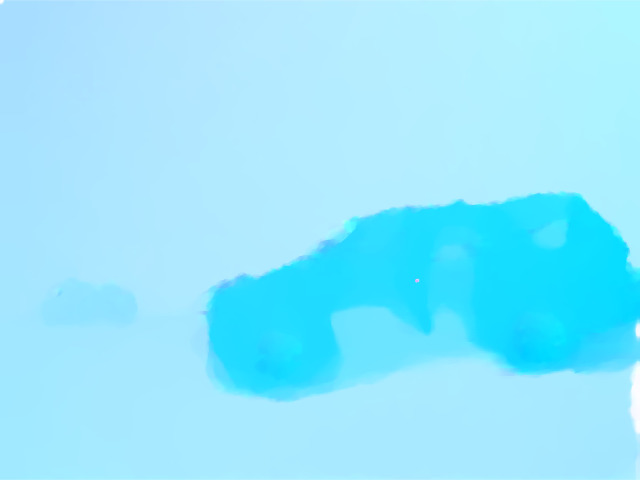
\includegraphics[width=0.48\linewidth] {implementation/flow_var/ff_c14_1}
   \label{fig:c14_fv_flow}
}
\subfigure[Variance Field]{
   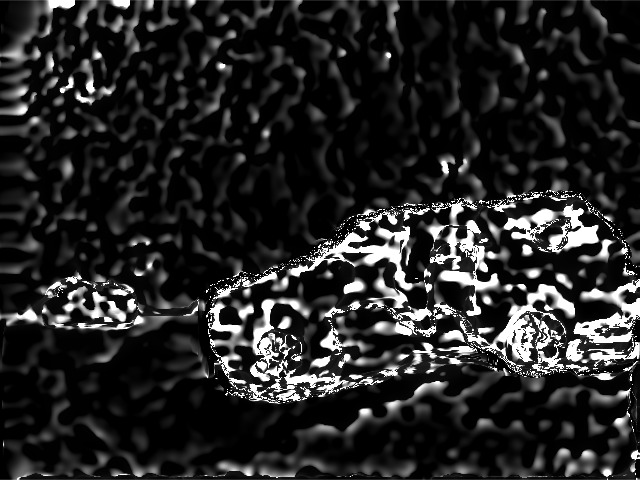
\includegraphics[width=0.48\linewidth] {implementation/flow_var/fv_c14_1}
   \label{fig:c14_fv_var}
}
\end{center}
\caption[Flow Variance]{Visualization of the flow variance computed by applying a bilateral filter on the optical forward flow.}
\label{fig:flow_variance}
\end{figure}
A detailed derivation of Equation $\ref{eq:flow_var_opt_flow}$ can be found in the appendix in Section $\ref{sec:derivation_flow_var}$ on page $\pageref{sec:derivation_flow_var}$.

\section{Trajectory Tracking}
\label{sec:trajectory_tracking}
As mentioned previously, motion is a spatially and temporally coherent visual cue. This implies that motion is not frame-wise independent and thus represents the history of every image location. In particular the motion history of a tracking candidates can be formed by tracing them to their successor frames using the optical flow. Another commonly used term for a point history is \textit{motion trajectory}. A trajectory is an ordered list of points produced by tracking an initial feature location over a series of frames. We conclude that every trajectory has a temporal aspect (the frames its tracking points correspond to) and a spatial aspect (the image locations its tracking positions map to). \\ \\
So far we have discussed how to obtain starting positions of trajectories (Sec. $\ref{sec:tracking_candidates}$) and when we have to stop them (Sec. $\ref{sec:occlusion_det}$). Moreover, by relying on the generated optical flow (Sec. $\ref{sec:generate_of}$) we are able to determine the location a point gets tracked to in its successor frame. Therefore, we are now able to discuss how to track motion trajectories. \\ \\
In this section we explain, in detail, the required steps to track motion trajectories. Moreover we discuss a transformation that allows us to obtain 3D world coordinates from the traced 2D trajectory points. For this purpose we will make use of the depth field.

\subsection{Point Tracking}
Every point $p_t$ in frame $t$ can be tracked to a position $p_{t+1}$ in its successor frame $t+1$ by using the corresponding forward flow field $w_t$ that belongs to frame $t$. This is achieved by adding $w_t$ to $p_t$, which yields $p_{t+1}$. We repeat this procedure until the point gets either occluded or has reached the last video frame. Algorithm $\ref{alg:point_tracking}$ offers a detailed description of the involved steps to run the point tracking. \\ \\
\begin{algorithm}[H]
\caption{Point Tracking}
\begin{table}[H]
  \begin{tabular}{@{}lll@{}}
    \textbf{Input:} & Tracking candidates \\
    	& Forward Flow fields $\textbf{F}$ \\
        & Occluded Regions \\
	\textbf{Output:} & Trajectories $\textbf{T}$
  \end{tabular} 
\end{table}
\setlength{\fboxrule}{0pt} 
\begin{boxedminipage}{1.0\textwidth}
  \begin{algorithmic}[1]
  	\State $T \leftarrow \text{Initialize an empty list of trajectories}$
  	\State $\bar{T} \leftarrow \text{Initialize an empty list of trajectories}$
  	\For{$k=1 \text{ TO FrameCount}$}
  		\State $C \leftarrow \text{load all tracking candidates that belong to frame } k$
  		\State $\text{Start a new trajectory for each candidate and append it to T}$

  		\ForAll{$\text{Trajectory } t \in T \text{ that has not ended yet}$}
  			\State $p \leftarrow \text{getPointAtFrame(k)}$
  		  	\State $\text{Fetch forward flow vector fv} = \textbf{F} \left(k, p \right)$
  			\State $\text{Compute the tracked to position: } tp = p + fv$
  			\If{$tp \text{ lands in occluded region}$} 
  				\State $\text{End tracking of trajectory } t $
  				\State $\bar{t} \leftarrow \text{Start a new trajectory using tp as starting position}$
  				\State $\text{Append } \bar{t} \text{ to } \bar{T}$
  			\Else 
  				\State $\text{Append tp to trajectory t}$
  			\EndIf
  		\EndFor
  		\State $\text{Move all trajectories in } \bar{T} \text{ to T}$
    \EndFor
  \end{algorithmic}
  \end{boxedminipage}
  \vskip1.5pt
\label{alg:point_tracking}
\end{algorithm}
$\newline$
The point tracker algorithm consists of two main loops. The outer loop iterates over the number of frames present in the selected dataset and the inner loop runs over the set of all trajectories. First, we load all corner candidates, the occlusion maps and the generated flow fields into our pipeline. Then, we initialize an empty trajectory set. \\ \\
In every outer loop iteration we load all tracking candidates that correspond to the current frame index and use them to start new trajectories. Starting a new trajectory by a point means to use that given point as the trajectory's first tracking point. In addition, we also store the frame index to which this point belongs to. Moreover, every new started trajectory is marked as not closed, meaning that it can be used to continue its tracking. Only trajectories that were tracked to occluded regions get marked as closed. \\ \\
Next, we proceed with the in the inner loop, which runs the actual point tracking. We select every trajectory that is currently not marked as closed. For each such trajectory we first load its last appended tracking point. Moreover, the flow vector that matches the current trajectory point is loaded. Next, we compute a potential tracked-to position by adding the forward flow vector to the tracking point. We use the wording \textit{potential}, because we have to check first, whether this point was tracked to an occluded region. \\ \\
In case the point was not occluded, we append the computed tracked to position to the trajectory and continue to track the next trajectory. Otherwise, if the point was traced to an occluded region, we have to end the tracking of the currently considered trajectory and mark it as closed. The tracking has to be stopped as soon as a point gets occluded, otherwise the trajectory will share the motion of two different objects. \\ \\
In the occluded case, the computed tracked to position is then used to start a new trajectory. Doing so solves the problem of disocclusion, because empty areas, that are not yet covered by trajectories, get filled. \\ \\
This procedure is repeated until we have processed every frame and trajectory. \\ \\
Finally, we conclude this section by offering an example of an actual point tracking applied on the cars dataset. The resulting trajectories, as well as their tracking points, are shown in Figure $\ref{fig:cars_trajectories}$. In this visualization we see different trajectories, tracked over four frames. Tracking points that belong to the same trajectory have the same color as their trajectory. As we can see, points that were tracked along the same moving objects exhibit consistent trajectories. In other words, our flow field based tracker produces reliable and meaningful results in this example.
\begin{figure}[H]
\begin{center}
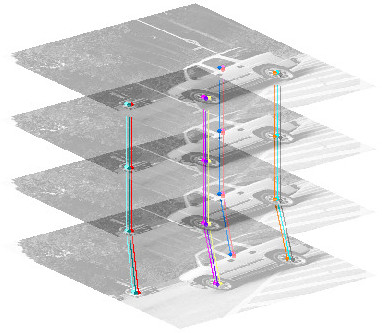
\includegraphics[width=0.65\linewidth] {implementation/trajectories/cars_trajectories_4_sel}
\end{center}
\caption[Trajectories]{Exemplary trajectories tracked in the Cars$\footnotemark$ dataset shown in different color. The tracking points exhibit the same color as the trajectory they belong to. The tracking points are plotted as thick dots.}
\label{fig:cars_trajectories}
\end{figure}
\footnotetext{To generate Figure $\ref{fig:cars_trajectories}$ I used the Cars dataset from the BMS-26 dataset: Source\\ 
\url{http://lmb.informatik.uni-freiburg.de/resources/datasets/}}

\subsection{Transformation to 3D Points}
\label{subsection:transform_to_3d_points}
In the previous section we described a method to run a tracking of motion trajectories. However, the so far traced trajectories consist of a set of 2D dimensional tracking points, since both, the optical flow fields and our tracking candidates, are defined over the 2D image space. Ideally, for defining more accurate similarities between trajectories we would like to use 3D versions of the trajectory points instead. Therefore we have to transform our extracted motion trajectories so that they are defined in the 3D world space. To define such a transformation we have to make use of the depth fields and the camera calibration. \\ \\
In the following section we explain how such a transformation from 2D image space to 3D world space can be implemented. We assume, that the utilized RGBD-video sequences were captured using two cameras, a color and depth camera. To be as general as possible, we further assume that these cameras are not aligned. Having a formulation based on this assumptions allows us to support a broad series of video sequences captured by various devices. \\ \\
Let us model the two cameras by a pinhole camera as described in the appendix Section $\ref{sec:pinhole_camera}$. The pinhole camera model is a simple mathematical model to define a projection from the world space to the 2D image space using a homogeneous transformation defined as: 
\begin{equation}
\colvec[f_x X + Z p_x]{f_y Y + Z p_y}{Z} =
\begin{bmatrix}
f_x & 0 & p_x & 0 \\
0 & f_y & p_y & 0 \\
0 & 0 & 1 & 0
\end{bmatrix}
\begin{pmatrix}
X \\
Y \\
Z \\
1
\end{pmatrix}
\label{eq:homogen_camera_mat_transf}
\end{equation}
where given the  $p = \left(p_x, p_y \right)$ denotes the principal point and the focal lengths $\left(f_x, f_y \right)$ of the camera. \\ \\
So far we have exactly the opposite of what we would like to get: We defined a transformation that allows to project a 3D point onto the 2D image space. However, deriving the inverse transformation of the definition of Equation $\ref{eq:homogen_camera_mat_transf}$ allows us to define points in the 3D space. In the following, let us assume that $z$ denotes measured depth $d$. Then
\begin{equation}
	\colvec[X]{X}{Z} \mapsto \left( \frac{f_x x}{d} + p_x, \frac{f_y y}{d} + p_y \right)^T
\end{equation}
since
\begin{equation}
\begin{aligned}
	d \left( \frac{x - p_x}{f_x} \right) = \hat{x} \Leftrightarrow \frac{\hat{x}}{d} f_x + p_x = x \\
	d \left( \frac{y - p_y}{f_y} \right) = \hat{y} \Leftrightarrow \frac{\hat{y} f_y}{d} + p_y = y 
\end{aligned}
\label{eq:depth_tranfomation}
\end{equation}
The aspect that color and depth cameras are not aligned can be modeled by defining an extrinsic calibration matrix $E$. Such a matrix defines how a camera has to be shifted and rotated to align with another camera. Given the extrinsic and intrinsic camera calibration data this is defined as
\begin{equation}
\begin{aligned}
	\text{Camera}^{depth} : \left( p^d = (p_x^d, p_y^d), f^d = (f_x^d, f_y^d)\right) \\
	\text{Camera}^{color} : \left( p^c = (p_x^c, p_y^c), f^c = (f_x^c, f_y^c)\right) \\
	\textbf{E} : \text{Camera}^{depth} \rightarrow \text{Camera}^{color}
\end{aligned}
\label{eq:calib_data}
\end{equation}
In order to transform a 2D pixel coordinate $\left( u, v \right)$ (in image space) to a 3D world coordinate $\left( x, y, z \right)$ we have to run the following steps:
\begin{enumerate}
\item Transform image location onto depth camera space:
\begin{equation}
	\forall (u, v), \forall d = \textbf{D}(u,v): \colvec[\frac{u - p_x^d}{f_x^d} d]{\frac{v - p_y^d}{f_y^d} d}{d} = \colvec[x]{y}{z} \equiv \bf{p}
\end{equation}
\item Align depth camera with the color camera by applying the extrinsic matrix $E$:
\begin{equation}
	\forall p: \hat{p} \equiv \colvec[\hat{x}]{\hat{y}}{\hat{z}} =  E p
\end{equation}
\item transform the points onto color camera
\begin{equation}
	\forall \hat{p} : \left( \hat{u}, \hat{v}\right) = \colvec{\frac{\hat{x}}{\hat{z}} f_x^c + p_x^c}{\frac{\hat{y}}{\hat{z}} f_y^c + p_y^c}
\end{equation}
\end{enumerate}

\section{Affinity Matrix Generation}
\label{sec:affinity_matrix_impl}
In this section we describe the corresponding pipeline stage that is responsible for generating the so called $\textit{affinity matrix}$, which is later used to compute the actual motion segmentation. For this purpose we compute the pairwise similarities between the previously tracked trajectories according to a certain measure and then use those values to form a similarity graph as defined in Section $\ref{sec:similarity_graphs}$ on page $\pageref{sec:similarity_graphs}$. However, computing affinities based on pairwise trajectory distances corresponds to assuming a translational motion model. Especially in real world examples objects usually form affine motions $\footnote{An affine motion requires to compute distances on trajectories at a time to verify if it belongs to the a certain motion group.}$ and thus this assumption is imposing a certain error. Despite this limitation we will present a robust solution to this issue. \\ \\
The final affinity matrix correspond to the adjacency matrix representation of the similarity graph. The used metrics are adapted versions of the metrics presented in $\cite{OB14b}$ and $\cite{KB15b}$. \\ \\
In general, trajectories of longer videos are asynchronous, i.e. they cover different temporal windows in a shot. Furthermore, the number of points that are tracked across the whole image sequence is small or even empty due to occlusion, disocclusion or the sampling rate. Hence, a measurement matrix that utilizes the coordinates of the tracked points, as used by the multi-body factorization and subspace methods, will have many missing entries and thus is a bad choice. However, there is a remedy to this issue. We, instead, compute pairwise affinities between trajectories, because this only requires some trajectories to have some temporal overlap. In particular, we define affinities between all pairs of trajectories that share at least a common frame. \\ \\
According to the gestalt principle of common fate$\footnote{Human tend to group similar objects together that share a common motion.}$, we should assign high affinities to pairs of points that move together. Imagine the situation where two persons are walking next to each other$\footnote{Assume both persons are walking at the same speed in the same direction, ignoring all motions due to deformation.}$. Although they represent different objects, both of them share the same motion. Moreover, a person that sits still in a chair shares the same motion as the objects in the background. The gestalt principle tells us that these situations should be treated conservatively and the objects from these examples should not be separated. \\ \\
In the following we describe in detail the steps of Algorithm $\ref{alg:computing_affinity_matrix}$ which is used to generate the affinity matrix.
\begin{algorithm}[H]
\caption{Generating Affinity Matrix}
\begin{table}[H]
  \begin{tabular}{@{}lll@{}}
    \textbf{Input:} & Extracted Trajectories \bf{T} \\
		& Forward Flow Fields \bf{OF} \\
 		& Dataset Images (\emph{optional}) \bf{F} \\
    \textbf{Output:} & Affinity Matrix \bf{W} \\
    & Nearest Trajectory Neighbors \bf{$\mathcal{N}$}\\
    & Trajectory Labels \bf{$\mathcal{L}$}\\
  \end{tabular} 
\end{table}
\setlength{\fboxrule}{0pt} 
\begin{boxedminipage}{1.0\textwidth}
  \begin{algorithmic}[1]
      \State $\text{Form every possible trajectory pair combination of } \bf{T}$
      \State $\text{Filter too short trajectories}$
      \ForAll{$\text{Trajectory pair } \left( \textbf{a}, \textbf{b} \right)$}
        \State $\left( \textbf{p}^a, \textbf{p}^b \right) \longleftarrow\text{Select all temporal overlapping segments between } \textbf{a} \text{ and } \textbf{b}.$
        \State $d_{\text{spatial}} = \text{computeSpatialDistance}\left( \textbf{p}^a, \textbf{p}^b, \textbf{T} \right)$
        \State $d_{\text{color}} = \text{computeColorDistance}\left( \textbf{p}^a, \textbf{p}^b, \textbf{F} \right)$
        \State $d_{\text{motion}} = \text{computeMotionDistance}\left( \textbf{p}^a, \textbf{p}^b, \textbf{F} \right)$
        \State $d^2 = \text{combineDistances} \left( d_{\text{spatial}}, d_{\text{color}}, d_{\text{motion}} \right)$
        \State $W \left( \textbf{a}\text{.label}, \textbf{b}\text{.label} \right) = e^{-\lambda d^2}$
        \State $\text{Update nearest neighbors of } \textbf{a} \text{ and } \textbf{b} \text{ using } d_{\text{spatial}}$
      \EndFor
  \end{algorithmic}
  \end{boxedminipage}
  \vskip1.5pt
\label{alg:computing_affinity_matrix}
\end{algorithm}
As the very first step, our pipeline loads the previously extracted trajectories into its memory. Each loaded trajectory gets a unique identifier, which is called $\textit{label}$, assigned. Next, we discard every trajectory that is shorter than a user specified threshold to reduce the effect of noisy and invalid tracings. From the remaining trajectories we form every possible pair combination and compute certain distances between them as illustrated in Figure $\ref{fig:distance_measure}$.
\begin{figure}[H]
\begin{center}
\subfigure[Overlapping Trajectories]{
   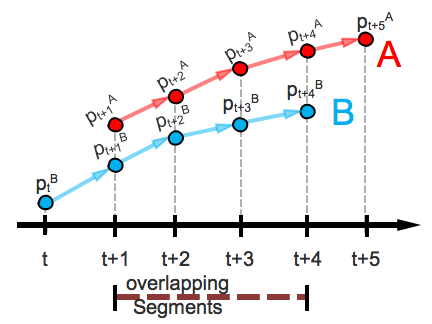
\includegraphics[width=0.7\linewidth] {implementation/affinities/overlapping_tra}
   \label{fig:overlapping_tra}
}
~
\subfigure[Color Distance]{
   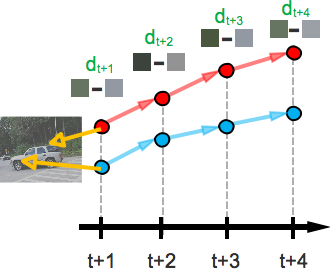
\includegraphics[width=0.3\linewidth] {implementation/affinities/d_co}
   \label{fig:tra_distance_measures_co}
}
\subfigure[Motion Distance]{
   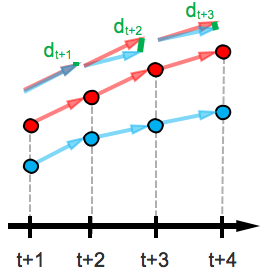
\includegraphics[width=0.3\linewidth] {implementation/affinities/d_mo}
   \label{fig:tra_distance_measures_mo}
}
\subfigure[Spatial Distance]{
   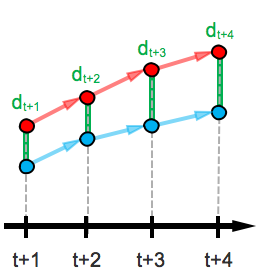
\includegraphics[width=0.3\linewidth] {implementation/affinities/d_sp}
   \label{fig:tra_distance_measures_sp}
}
\end{center}
\caption[Distance Measures]{For a given trajectory pair $(A,B)$ we compute their spatial (Fig. $\ref{fig:tra_distance_measures_sp}$), color (Fig. $\ref{fig:tra_distance_measures_co}$), and motion (Fig. $\ref{fig:tra_distance_measures_mo}$) distances between their overlapping segments.}
\label{fig:distance_measure}
\end{figure}
For any two given trajectories $A$ and $B$ that form a pair, our pipeline computes the following three distances between their temporal overlapping segments$\footnote{By the term \textit{temporal overlapping segments} we refer to tracking point in a trajectory pair that share a common frame.}$:
\begin{itemize}
\item The \textbf{spatial distance} $d_{\text{spatial}}$: Trajectories that belong to the same object are usually spatially close to each other and are defined as
\begin{equation}
	d_{spatial}^{A,B} = \frac{1}{\omega - \alpha + 1} \sum_{k=\alpha}^\omega \norm{A(k) - B(k)}
\label{eq:spatial_distance}	
\end{equation}
where $\alpha$ is the first- and $\omega$ is the last- overlapping frame index between the two given trajectories $A$ and $B$.
\item The \textbf{color distance} $d_{\text{color}}$: Within a certain object region, associated trajectories are tracked at locations that have a similar color value. This distance is defined as:
\begin{equation}
	d_{color}^{A,B} = \frac{1}{\omega - \alpha + 1} \sum_{k=\alpha}^\omega \norm{\text{ColorAt}(k, A(k)) - \text{ColorAt}(k, B(k))}_2
	\label{eq:color_dist}
\end{equation}
where $\text{ColorAt}(k, A(k))$ yields a color in \textit{Cielab} color space$\footnote{Using Cielab colors enables us to use the l2 norm in order to compute color distances.}$ value in frame $k$ at the image location $A(k)$.
\item The \textbf{motion distance} $d_{\text{motion}}$: The rationale of this measure is to exploit$\footnote{Again, thanks to the gestalt principle of common fate we know that for each pair of trajectories at the time instant where their motion is maximally different, the two points do not belong to the same object,}$ the maximal dissimilarity of the two given trajectories via their maximal motion difference among all overlapping frames. The motion distance is defined as
\begin{equation}
	d_{motion}^{A,B}  = \max_t \left( \frac{\norm{\partial_t A - \partial_t B}}{\sigma_t} \right)
\label{eq:motion_distance}
\end{equation}
where the expression $\partial_t A$ denotes the averaged motion over time, which is defined as 
\begin{equation}
	\partial_t A = \frac{A(t+T)-A(t)}{T} 
\end{equation}
The exact value of $T$ is the minimum of the number of overlapping frames between $A$ and $B$ and a fixed threshold. In our pipeline we use $T$ equals 3. Furthermore, the resulting motion distance is normalized by its corresponding flow variance value $\sigma_t$. The idea is to reduce the influence of noise, which is present in the estimated flow fields. Especially, when taking differences between flow vectors, the noise level could get even more amplified. Additional information about this normalization, as well as the definition of this variance can be found in Section $\ref{sec:flow_variance}$ on page $\pageref{sec:flow_variance}$.

\end{itemize}
Note that $A(k)$ denotes the tracking position of trajectory $A$ in frame $k$. The final similarity between two trajectories is the combination of these distances according to a user-specified combination method. Therefore, let us introduce these combination methods that are supported by our pipeline. \\ \\
There are two main settings a user has to specify preliminarily (Fig. $\ref{fig:affinity_modes}$): Whether or not depth cues should be used and how the computed distances should be combined to define an affinity value between trajectories. Both options have a large impact on the final outcome of the affinity matrix. \\ \\
First, when enabling depth cues, all available depth fields are loaded into the pipeline. In combination with the depth- and color-camera calibration data, this enables the pipeline to compute the three dimensional version of each traced trajectory point, analogous as described in the previous Subsection $\ref{subsection:transform_to_3d_points}$ on page $\pageref{subsection:transform_to_3d_points}$. As a direct consequence, when using depths, the spatial distance computation is altered. Instead of using the 2D tracking points, we use their 3D transformed versions, computed as explained in Section $\ref{subsection:transform_to_3d_points}$. \\ \\
Furthermore, our pipeline supports two distance combination methods: Either it combines them by calculating the weighted sum of the distance values $\cite{KB15b}$ or it multiplies all the distances $\cite{OB14b}$. Depending on the used combination strategy, different segmentation methods have to be used later on. Summed distances can only be used in combination with the $\textit{Kernighan-Lin}$ segmentation method (Sec. $\ref{sec:kl_impl}$), whereas the product of distances can be either used in our \textit{Spectral Clustering} (Sec. $\ref{sec:spectral_clustering_impl}$) or \textit{Minimum Cut} segmentation (Sec. $\ref{sec:min_cut_seg}$) method$\footnote{The reason for this limitation is due to the fact that similarity matrices used by spectral clustering algorithms are supposed to have non-negative entries. However, the summed distances combination method may yield negative weights and thus some entries in the similarity matrix might be negative. Further information about this limitation can be found in $\cite{Lux07}$}$. \\ \\
In the beginning of this section, we stated, that our pipeline assumes a translational motion model. This is due to the fact that we compute pairwise distances between trajectories. However, affine motions can locally be approximated by a translation. Therefore, our idea is to damp the effect of model noise by scaling the affinities by their spatial distances. The further two trajectories are apart from each other, the less reliable their local approximation is. Both distance combination method will implement this damping idea in a certain way. In the following we offer an in depth explanation about these combination variants:
\paragraph{Summed Distances}: This combination method computes a weighted sum of the spatial-, color- and motion distance and is defined as
\begin{equation}
\begin{aligned}
z ( A, B ) = \max (\tilde{\beta_0} & + \beta_1 d_{motion}^{A,B} \\
& + \beta_2 d_{spatial}^{A,B} \\
& + \beta_3 d_{color}^{A,B},\\
\beta_0 & + \beta_1 d_{motion}^{A,B} )
\end{aligned}
\label{eq:sum_dist}
\end{equation}
If the sum of the spatial and the color distance is large in Equation $\ref{eq:sum_dist}$ then only the motion distances are considered. This ensures that trajectories, which are far apart but move similarly, still end up in the same segment. For assigning the beta parameters in Equation $\ref{eq:sum_dist}$ we use the same values as defined in $\cite{KB15b}$.\\ \\
This combination function yields arbitrary values in the positive real numbers, i.e. positive values. This combination strategy returns an affinity matrix that is dedicated to the $\textit{Kernighan-Lin}$ segmentation implementation. Affinities generated by this combination strategy are referred to as \textbf{S-affinities}.
 
\paragraph{Multiplied Distances}: This combination method multiplies the spatial and motion distance according to the following definition:
\begin{equation}
	d^2 \left( A, B \right) = d_{spatial}^{A,B} \left( d_{motion}^{A,B} \right) ^2
\label{eq:prod_combination}
\end{equation}  
The resulting distance value from Equation $\ref{eq:prod_combination}$ is then turned into an affinity via the transformation
\begin{equation}
	w \left( A, B \right) = e^{ -\lambda d^2 (A, B) }.
	\label{eq:prod_dist_affinity}
\end{equation}
This combination function always yields values between zero and one. A value close to one means, that the two trajectories are very similar, whereas a value close to zero or even equals zero means that they are very distinct according to the used metrics. Moreover, if the spatial distance dominates, the affinity becomes very small. Hence, the further away two trajectories are, the less similar they are. This preserves our local motion model assumption. \\ \\
The measure from Equation $\ref{eq:prod_dist_affinity}$ is based on the work of Shepard $\cite{Shepard87}$ who proposed a universal law that distance and perceived similarity are related via an exponential function. The scalar $\lambda$ acts as a scaling factor and has to be specified by the user$\footnote{We found that when running PD, then $\lambda$ equals 0.1 is a good choice and when running PED $\lambda$ equals 10 produces good results.}$. Affinities generated by this combination strategy are referred as \textbf{P-affinities}. \\ \\
Our pipeline implements four affinity matrix generation modes. These available pipeline modes are a direct consequence of the possible user choices between the questions \textit{"should we use depths or not?"} and \textit{"should we combine distances according to Equation $\ref{eq:prod_dist_affinity}$ or Equation $\ref{eq:sum_dist}$?"}. In this thesis, we use the following abbreviations: \textbf{PD} and \textbf{PED} stand for product of distances, whereas the additional \textit{E} in PED stands for \textit{euclidean} and hints that we are using 3D points in meter units instead of pixel units. Similarly, \textbf{SD} and \textbf{SED} stand for \textit{summed} (euclidean) distances. A graphical representation of these modes is given in Figure $\ref{fig:affinity_modes}$.
\begin{figure}[H]
\begin{center}
   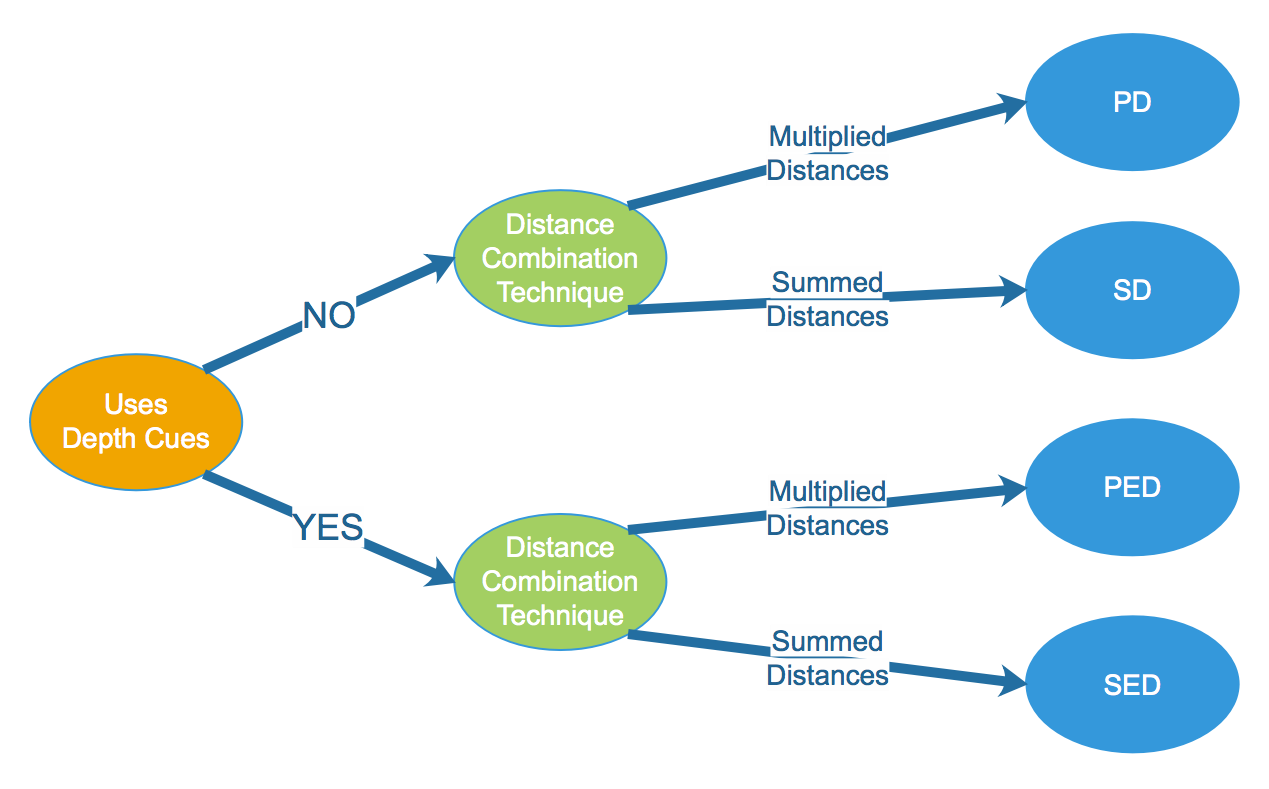
\includegraphics[width=0.7\linewidth] {implementation/affinities/modes}
\end{center}
\caption[Affinity Pipeline Modes]{A visualization of all affinity computation modes that can be run by our pipeline. The PD mode corresponds to the distance measure described in $\cite{OB14b}$ and SD to the measure described in $\cite{KB15b}$. However, the modes PED and SED, which incorporate depths, are novel approaches. In our pipeline we use PD and PED to run the spectral clustering (Sec. $\ref{sec:spectral_clustering_impl}$)} or the mincut (Sec. $\ref{sec:min_cut_seg}$) segmentation methods. Moreover, the modes SD and SED are used by the Kernighan-Lin graph partitioning method (Sec. $\ref{sec:kl_impl}$).
\label{fig:affinity_modes}
\end{figure}
Additionally, our pipeline also offers a mode to compute affinities between shortly disconnected trajectories. The idea is to prepend (extend) one additional tracking point to a predecessor (successor) frame by adding the average motion distance of the next (previous) five frames to the trajectory's starting point (end point). Please note that this run-mode is only optional and thus has to be invoked manually. Moreover, we could not observe any improvements in the resulting segmentations, when enabling this mode. \\ \\ 
In summary, the affinity matrix is computed between a trajectory and every other trajectory by calculating the distances described above and then combining them in a certain way. Every trajectory instance, therefore, carries a list of affinities, which are sorted by their partner trajectory's label in an ascending order. \\ \\
Therefore, for building the affinity matrix, we fetch all used trajectories and order them by their label value (again, ascending). Then, all we have to do is to traverse these ordered trajectories and then write their ordered affinities (to the other trajectories) into a file. Actually, each trajectory forms a line, where a line consists of the affinity values of the currently visited trajectory. Our writer uses a special file formatter that is able to generate a Matlab readable file. The pairwise affinities for $n$ valid trajectories result in a $n \times n$ affinity matrix $W$ as shown in Figure $\ref{fig:cars_affinity_matrix}$. \\ \\
\begin{figure}[H]
\begin{center}
   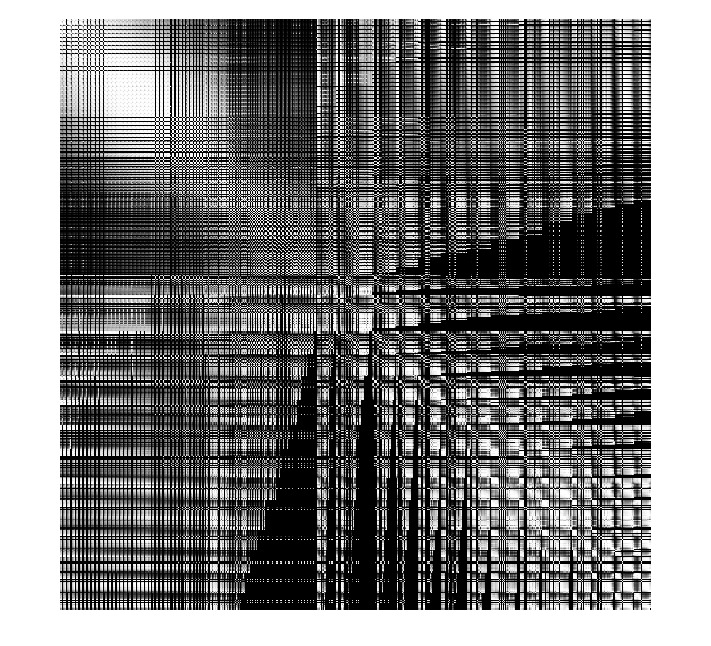
\includegraphics[width=0.65\linewidth] {implementation/affinities/cars/cars_w}
   \label{fig:cars_w}
\end{center}
\caption[Affinity Matrix]{Visualization of affinities among trajectories and the structure of their matrix $W$. The affinity is visualized by a grayscale image. The row-and column indices in the matrix determine a trajectory pair and the value at that position corresponds to their affinity. Bright values indicate a high affinity between two trajectories.}
\label{fig:cars_affinity_matrix}
\end{figure}
To support later queries that allow to fetch affinities by a trajectory label, we also have to write a file containing all valid trajectory label identifiers. The labels are in an ascending order with respect to their label ID. Figure $\ref{fig:affinity_index_label_mapping}$ shows how an affinity lookup by two given trajectory labels can be performed.
\begin{figure}[H]
\begin{center}
   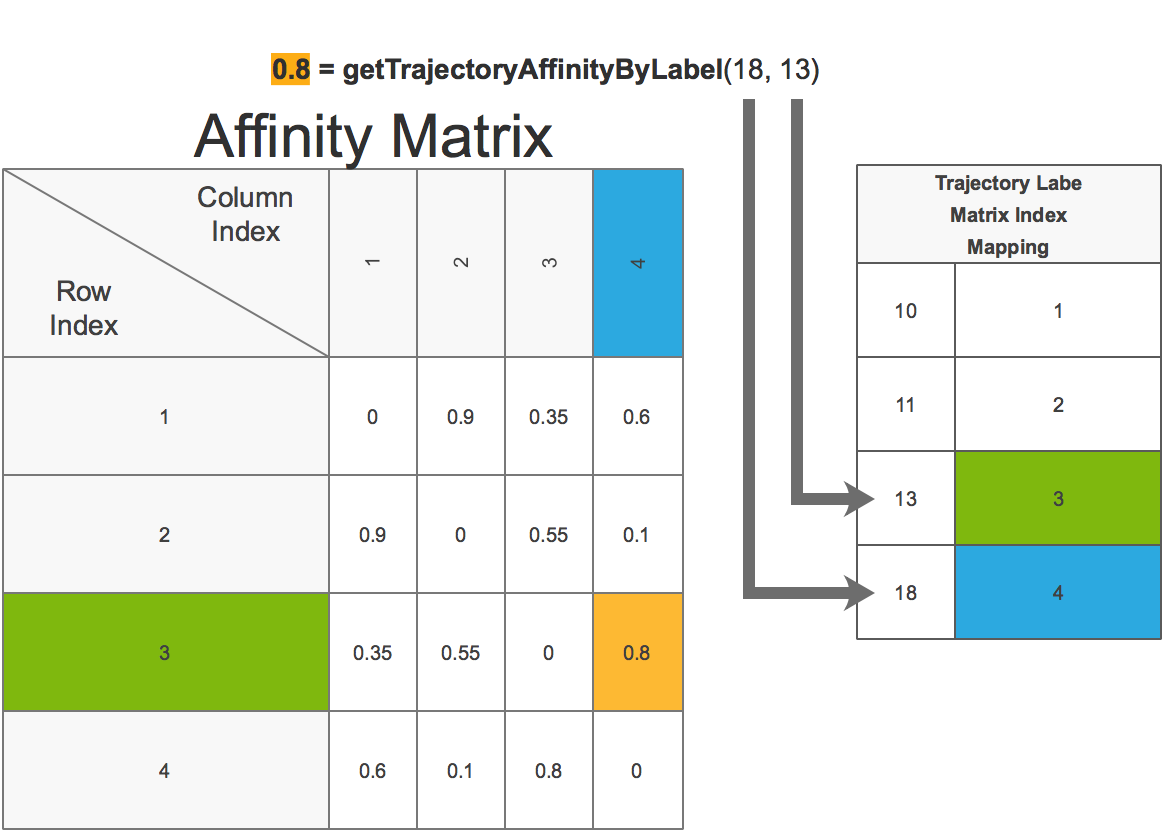
\includegraphics[width=0.85\linewidth] {implementation/affinities/affinity_label_mapping}
   \label{fig:cars_w}
\end{center}
\caption[Mapping between Affinity Matrix Indices and Trajectory Labels]{In order to lookup an affinity value between two trajectories, we first have to lookup their matrix indices. This is performed by loading a file that contains a mapping between the trajectory-labels and affinity matrix-indices. In this example, we want to get the affinities between the trajectories with the label ID 18 and ID 13. We first look at those label's matrix indices and then use those indices to look up the actual affinity value.}
\label{fig:affinity_index_label_mapping}
\end{figure}
Apart from generating the affinity matrix, our pipeline also extracts the per trajectory nearest neighboring trajectories. This neighborhood information is later used by some of our segmentation methods do define smoothness energies. The distance to those neighbors is measured with respect to the average spatial distance. Luckily, we already have computed this spatial distance value while traversing the trajectory pairs. \\ \\
To conclude this section and offer a better understanding what those affinities actually are and mean, we discuss an affinity visualization, produced by our pipeline, shown in Figure $\ref{fig:cars_affinities}$.
\begin{figure}[H]
\begin{center}
\subfigure[Similarities Car Foreground]{
   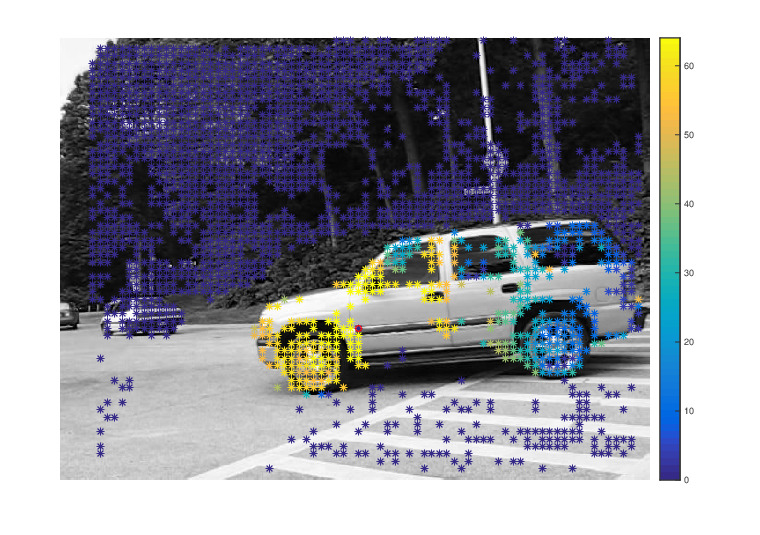
\includegraphics[width=0.48\linewidth] {implementation/affinities/cars/fc}
   \label{fig:cars_a}
}
\subfigure[Similarities Car Background]{
   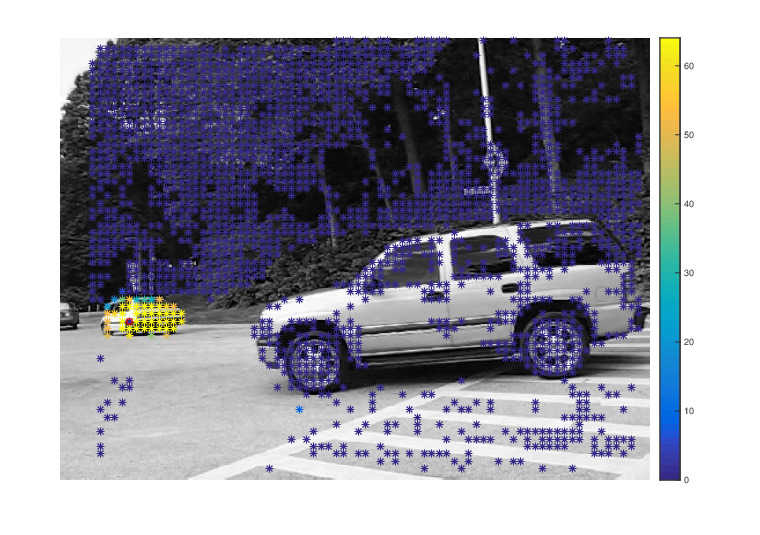
\includegraphics[width=0.48\linewidth] {implementation/affinities/cars/cb}
   \label{fig:cars_b}
}
~
\subfigure[Similarities Woods]{
   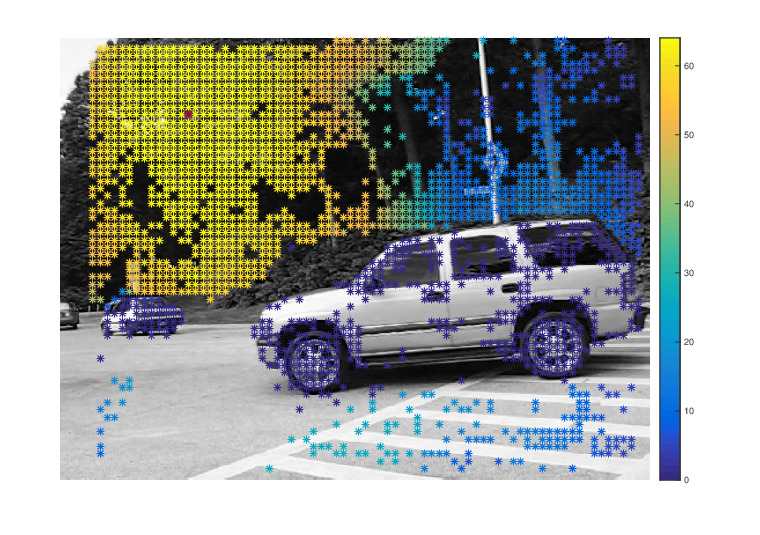
\includegraphics[width=0.48\linewidth] {implementation/affinities/cars/woods}
   \label{fig:cars_c}
}
\subfigure[Similarities Street]{
   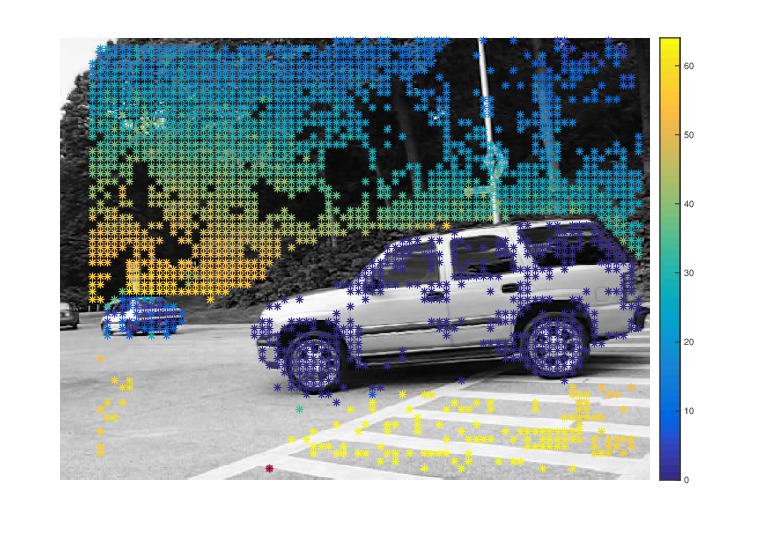
\includegraphics[width=0.48\linewidth] {implementation/affinities/cars/street}
   \label{fig:cars_d}
}
\end{center}
\caption[Trajectory Affinities Example]{Visualizing four examples$\footnotemark$ of the affinities between a selected trajectory point (marked in red) and its affinities to any other present trajectory point. The more similar two points are, the more yellowish a dot becomes. In contrast, the more dissimilar two points are, the more bluish the point becomes.}
\label{fig:cars_affinities}
\end{figure}
\footnotetext{Affinities of the Cars dataset from the BMS-26 dataset from\\ 
\url{http://lmb.informatik.uni-freiburg.de/resources/datasets/}}
In this figure, we visualize four examples of the affinity values between a selected point (marked by a red dot) and every other trajectory. The larger the similarity, the more yellow the color becomes and, vice versa, the smaller the affinity, the more blue it becomes. For example in Subfigure $\ref{fig:cars_b}$, we selected a point on the moving car in the background. It has strong affinities to tracked points within the car and small affinities to the front car and to the background. Similar results are shown in the other subfigures. Hence, these results hint to the potential of our pipeline. \\ \\
In the next section we will discuss several methods that use the previously generated outputs to compute a sparse motion segmentation.

\section{Sparse Motion Segmentation}
\label{sec:sparse_motion_segmentation}
In this section we explain how we generate sparse motion segmentations using the previously calculated affinity matrix. \\ \\
\begin{figure}[H]
\begin{center}
\subfigure{
   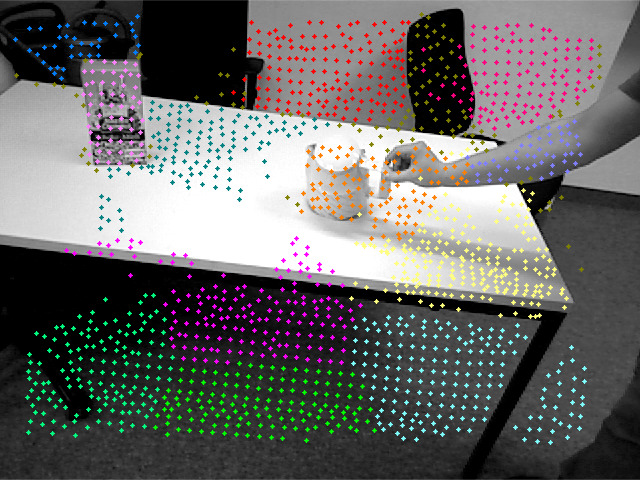
\includegraphics[width=0.31\linewidth] {implementation/segmentation/preword/bonn_cereal}
}
\subfigure{
   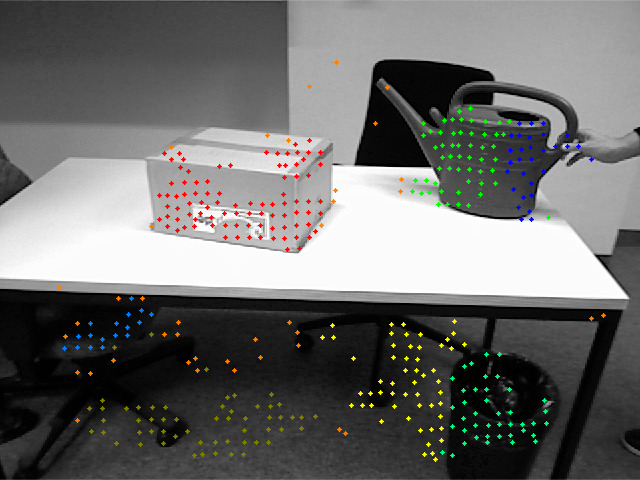
\includegraphics[width=0.31\linewidth] {implementation/segmentation/preword/bonn_watercan}
}
\subfigure{
   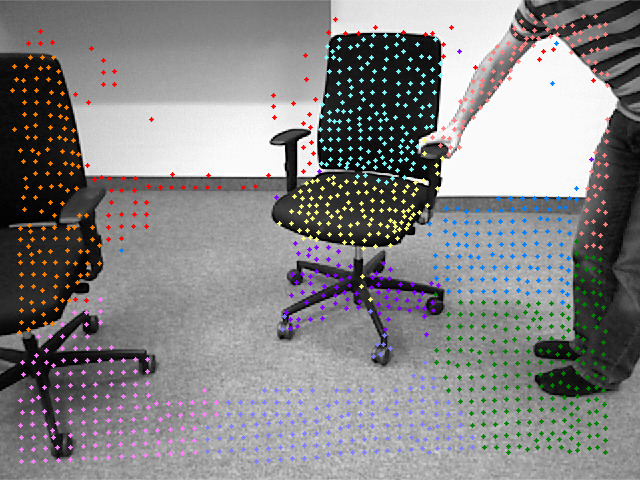
\includegraphics[width=0.31\linewidth] {implementation/segmentation/preword/bonn_chairs}
}
\end{center}
\caption[Sparse Segmentations]{Sparse motion segmentations$\footnotemark$ produced by our pipeline.}
\label{fig:sparse_segmentations}
\end{figure}
\footnotetext{Source of datasets used to generate the segmentations in Figure \ref{fig:sparse_segmentations}: \\ \url{http://www.ais.uni-bonn.de/download/rigidmultibody/}}
In fact, our pipeline supports three different segmentation methods, all having their pros and cons. In particular it can perform the task of motion segmentation using spectral clustering of the affinity matrix (\textbf{SC}), building a graph of the affinity matrix and calculating several cuts via min-cut (\textbf{MC}) or lastly, by using the affinities to solve the graph partitioning problem using the Kernighan-Lin Heuristic (\textbf{KL}). \\ \\
Every implemented segmentation method returns a file$\footnote{This enables us to draw the resulting motion segmentations.}$ containing a mapping between the trajectory label and their segment label. \\ \\
In order to draw the segmentation of the $k-th$ dataset frame, we load all trajectories that are active in that frame. For a trajectory, being active in a certain frame, refers to a trajectory, which contains a point that was tracked in that particular frame. To draw the segmentation image of frame $k$, we iterate over each trajectory and select their tracking points that are currently active in frame $k$. For each such tracking point we use its tracking position as the image location we want to draw a pixel\textit{draw to} at. Moreover, the label of its parent trajectory defines the color pixel color. Some resulting segmentations, produced by our pipeline, are shown in Figure $\ref{fig:sparse_segmentations}$.\\ \\
In the following we offer a detailed explanation of these motion segmentation methods.

\subsection{Spectral Clustering}
\label{sec:spectral_clustering_impl}
In the previous section we described how the pairwise affinities can be computed. For $n$ trajectories we ended up with a $n \times n$ affinity matrix $W$. \\ \\ 
One possible way to interpret these matrix entries is to identify them as edge weights of a fully connected graph $G$, where each trajectory represents a node. Following this interpretation, then, the task of extracting the moving objects  corresponds to the task of grouping several similar graph vertices. \\ \\
An approximately optimal partitioning of $G$ can be obtained via spectral clustering as described in Section $\ref{sec:spectral_clustering_bg}$. The idea behind this approach is to decompose the Laplacian matrix $L$ that corresponds to $W$ into its eigenvalues and eigenvectors $V$ and then to run k-means on $V$. We used Algorithm $\ref{alg:spectral_clustering_algorithm}$ in Matlab to run such a spectral clustering. As the first step we load the affinity matrix $W$ and compute its normalized Laplacian according to the definition from Equation $\ref{eq:normalized_graph_laplacian}$. Next, we compute the eigen-decomposition of $L$, defined as
\begin{equation}
	V^{T} \Lambda V = L^{\text{sym}}
\end{equation}
by using Matlab's fast eigen-decomposition $\textit{eigs}$. To get a better idea of how such eigenvectors might look like, please have a look at Figure $\ref{fig:eigenvectors_laplacian_matrix}$.
\begin{figure}[H]
\begin{center}
\subfigure[Eigenvector Front Car]{
   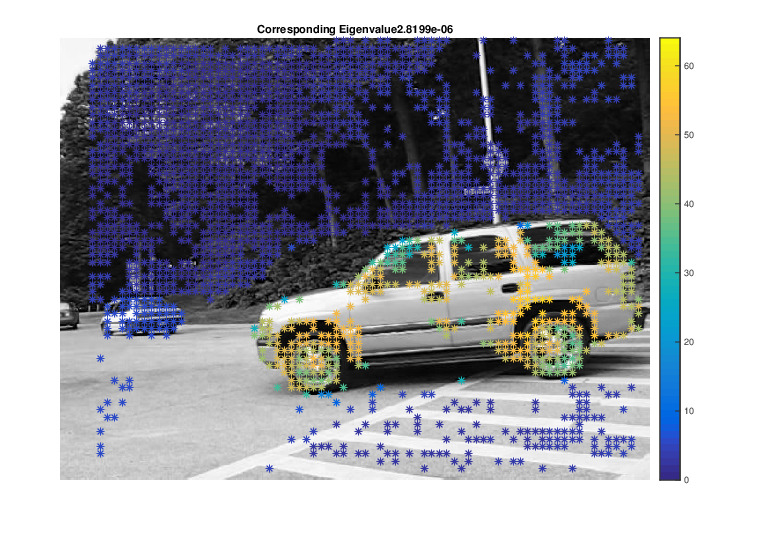
\includegraphics[width=0.48\linewidth] {derivation/eigenvectors/cars/ev_cf}
   \label{fig:cars_eigenvectors_laplacian_a}
}
\subfigure[Eigenvector Background Car]{
   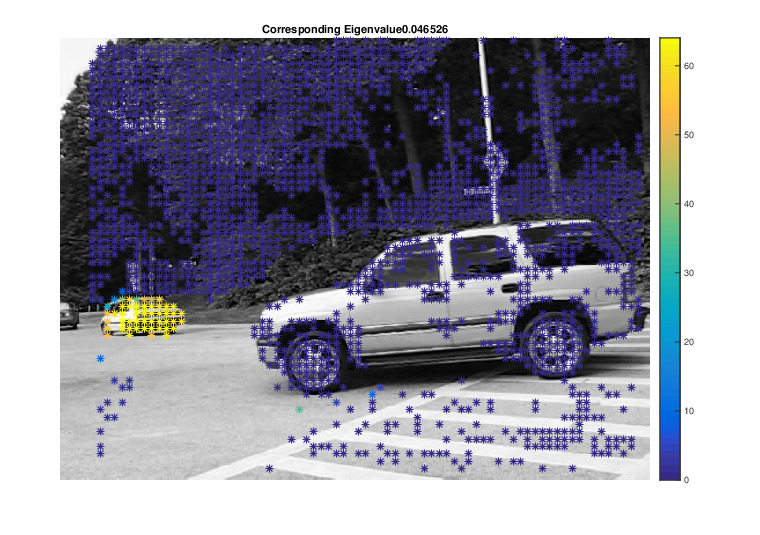
\includegraphics[width=0.48\linewidth] {derivation/eigenvectors/cars/ev_cb}
   \label{fig:cars_eigenvectors_laplacian_b}
}
\end{center}
\caption[Eigenvectors of Laplacian Matrix]{Visualizing the two smallest eigenvectors of the Laplacian matrix computed on the Cars$\footnotemark$ dataset. Each component of an eigenvector maps to exactly one trajectory. More yellow values indicate a large value, whereas bluish markings indicate a low value. The absolute value does not matter. However, we already observe local groupings of moving objects/their parts, when visualizing the eigenvectors.}
\label{fig:eigenvectors_laplacian_matrix}
\end{figure}
\footnotetext{Source of the Cars dataset: \\ 
\url{http://lmb.informatik.uni-freiburg.de/resources/datasets/}}
The actual clustering is performed on the eigenvectors of $L$. In fact, we further assume that we only need some of the eigenvectors for the clustering. Actually, it can be proven, that at least $k$ eigenvectors are required if there are $k$ segments$\footnote{In fact, the background is also counted as a segment. The actual proof shows, that to extract the k connected components in a graph, we need to run a spectral clustering on the k smallest eigenvectors.}$. Therefore, we select the $m$ smallest eigenvectors $V_m$ according to their $\lambda \in \Lambda$. \\ \\
The final clustering is performed by running k-means, similar as described in Section $\ref{sec:k_means}$, on $V_m$ using a pre-specified number of clusters. To run k-means, we use a random initialization. Since we might end up at a local minimum, we run the k-means algorithm 200 times and take the result with the smallest error$\footnote{The error is measured in terms of the distance between the resulting cluster centers and their assigned feature points.}$
The output of this method is a grouping of vector indices of the eigenvectors $V_m$. Each index \enquote{that belong to the same group} corresponds to the same moving object. To obtain the corresponding trajectory label that maps to a certain vector index, we perform a query similar as shown Figure $\ref{fig:affinity_index_label_mapping}$ by using the \textit{index-label-mapping} list. \\ \\ 
The actual choice for the number of $m$ and the clusters we want to solve for can be specified by the user. \\ \\
The limitation of this approach is that such a clustering is only defined for non-negative affinity values between trajectories. Otherwise the eigenvalue decomposition of the Laplacian would yield complex valued eigenvectors. In practice, this assumption means that it is easy to specify which trajectories should be in the same cluster but it is impossible to impose that they should be separated. Moreover, the described spectral clustering is supposed to produce oversegmentations and there is not always a smooth transition between the eigenvectors produced, when clustering them.

\subsection{Minimum Cut} 
\label{sec:min_cut_seg}
In this section we describe an alternative method to generate motion segmentation. This approach directly addresses some issues of the previously described spectral clustering approach. \\ \\
Typically, eigenvectors of the Laplacian matrix show smooth transitions within a region and more or less clear edges between regions. Unfortunately, the k-means algorithm cannot properly deal with this setting. Its results generally suffer from oversegmentations since it approximates smooth transitions by multiple constant functions. Furthermore, the optimal number of clusters $K$ is by no means obvious, because clusters are represented by many eigenvectors. \\ \\
To address this issue, we formulate an energy, similar as in $\cite{Bro10c}$, that comprises a spatial regularity term. By minimizing this energy term we obtain the optimal segmentation assignment. \\ \\
Initially, we again load the affinity matrix $W$, but this time together with the extracted trajectory's nearest neighbors $\mathcal{N}$. The actual number of trajectory neighbors is a user-tuneable parameter. The fewer neighbors a trajectory gets assigned to, the faster the pipeline runs. However, keep in mind that the number of neighbors determines the segmentation quality. Usually, one third of the total trajectory count is a solid choice for the neighborhood size. \\ \\ 
Analogously, as we did in the spectral clustering section, we transform $W$ to the normalized Laplacian and decompose it into its eigenvalues and eigenvectors. Again, the number of eigenvectors and clusters \enquote{we want to solve for} have to be specified by the user. \\ \\
In the following we describe this energy term, but before doing so, we have to provide the reader some definitions. Let $v_i^a$ denote the $a$-th component of the $i$-th eigenvector and $\textbf{v}^a$ the vector compose of the $a$-th components of all m extracted eigenvalues. Note that the index maps to a distinct trajectory. Let $\mathcal{N} \left( a \right)$ denote the neighboring trajectories of trajectory a, which were initially loaded. For a fixed number of clusters $K$, we want to compute the optimal trajectory assignments $\pi^{a} \in \{ 1, \dots , K \}$ such that the energy formulated in Equation $\ref{eq:min_cut_energy_revisited}$ is minimized.
\begin{equation}
\begin{aligned}
& E \left( \pi, K \right) = \underbrace{\sum_{A} \sum_{k=1}^K \delta_{\pi^A, k} \norm{\bf{v}^A - \mu_k}_{\lambda}}_\text{data term} + \underbrace{\nu \sum_A \sum_{B \in \mathcal{N}(A)} \frac{1- \delta_{\pi^A, \pi^B}}{\norm{\bf{v}^A - \bf{v}^B}}}_\text{smoothness term} \\
& \text{where } \norm{\bf{v}^A - \bf{\mu}}_\lambda = \sum \frac{v_i^A -  \mu_i}{\lambda_i}
\end{aligned} 
\label{eq:min_cut_energy_revisited}
\end{equation}
The $\delta_{\pi^A, \pi^B}$ is a characteristic function that is equal one, if the trajectories $A$ and $B$ are assigned to the same cluster and zero otherwise. Similarly, the expression $\delta_{\pi^A, k}$ is a boolean function that is one, if the trajectory $A$ got the label k assigned. \\ \\
The $\textbf{data term}$ models a unary cost that is minimized by k-means, where $\mu_k$ denotes the centroid of cluster $k$. Notice that this term makes use of the norm $\norm{.}_{\lambda}$. In this norm each eigenvector is weighted by the inverse of the square root of its corresponding eigenvalue. Such a weighting ensures that eigenvectors \enquote{that separate more distinct clusters} correspond to smaller eigenvalues. \\ \\
The $\textbf{smoothness term}$ acts as a regularizer that penalizes the spatial boundaries between clusters. The penalty is weighted by the inverse difference of the eigenvectors along these boundaries. On one hand, this penalty is very small for the case when there are clear discontinuities along cluster boundaries. On the other hand, boundaries within a smooth area are penalized more heavily. This avoids splitting clusters at arbitrary locations due to smooth transitions in the eigenvectors. \\ \\
The parameter $\nu$ acts as the trade-off between the two terms and thus determines how smooth the final segmentation should be. \\ \\
Minimizing the energy formulated in Equation $\ref{eq:min_cut_energy_revisited}$ is a difficult problem, because it exhibits many local minima. However, when using a fixed number of clusters $K$, minimizing this energy becomes a multi-label Markov Random Field (MRF) optimization problem with unknown centroids (see $\cite{TsaiBMVC10}$). Furthermore, in $\cite{Fulkerson2009}$ the authors have shown that such a multi-label MRF problem can be solved via max-flows. According to the Min-Cut-Max-Flow theorem $\cite{opac-b1078739}$ we can instead solve for the minimum cut. \\ \\
In our Matlab implementation we optimize this minimization problem by running an iterative solver as formulated in Algorithm $\ref{alg:final_min_cut}$. 
\begin{algorithm}[H]
\caption{Minimum Cut (\textbf{MC})}
\begin{table}[H]
  \begin{tabular}{@{}lll@{}}
    \textbf{Input:} & Cluster Count $k$ \\
    & Eigenvectors $V$ \\
    & Eigenvalue Count $m$ \\
    \textbf{Output:} & Assignments $(\pi_1, \dots, \pi_k)$ \\
  \end{tabular} 
\end{table}
\setlength{\fboxrule}{0pt} 
\begin{boxedminipage}{1.0\textwidth}
  \begin{algorithmic}[1]
  	  \State $\text{Initialize assignments } (\pi_1, \dots, \pi_k)$
      \Do
        \State $\text{Cluster centers } (\mu_1, \dots, \mu_k) \leftarrow \text{k-means}((\pi_1, \dots, \pi_k), V_m, k) \text{ (See Sec. }\ref{sec:k_means}\text{)}$
        \State $\text{Assignments } (\pi_1, \dots, \pi_k) \leftarrow \text{minCut}((\mu_1, \dots, \mu_k), V_m, k) \text{ (See Sec. }\ref{sec:graph_cut}\text{)}$
      \doWhile{$\text{Assignments have changed}$}
  \end{algorithmic}
  \end{boxedminipage}
  \vskip1.5pt
\label{alg:final_min_cut}
\end{algorithm}
Before starting the loop in Algorithm $\ref{alg:final_min_cut}$, we initialize the cluster centroids with an equidistant labeling (Fig. $\ref{fig:convergence_mc_seg_0}$) defined as
\begin{equation}
	\forall k \in \{ 1, \dots, K \} \forall A_i : (k - 1) \frac{n}{K} \leq i \leq k \frac{n}{K} : \pi^{A_i} = k
\label{eq:initialization_min_cut}
\end{equation}
A loop iteration consists of two main steps: First, we fix the label$\footnote{By the term \textit{labels} we are referring to the trajectory labels.}$ assignments and solve for the cluster centroids by running k-means (Sec. $\ref{sec:k_means}$). Next, we fix the centroids by using the previously computed centers and optimize for the assignments by running a multi-label graph cut (Sec. $\ref{sec:graph_cut}$) energy minimization. For this purpose we rely on $\cite{Fulkerson2009}$'s $\textit{GCMex}$ framework$\footnote{This frameworks offers some handy methods to compute the multi-label graph cut.}$, which is a freely available Matlab implementation. We repeat this iteration until the label assignments have converged. The resulting assignment is the motion segmentation. An example of the MC segmentation method is shown in Figure $\ref{fig:convergence_mc_seg}$.
\begin{figure}[H]
\begin{center}
\subfigure[Initialization]{
   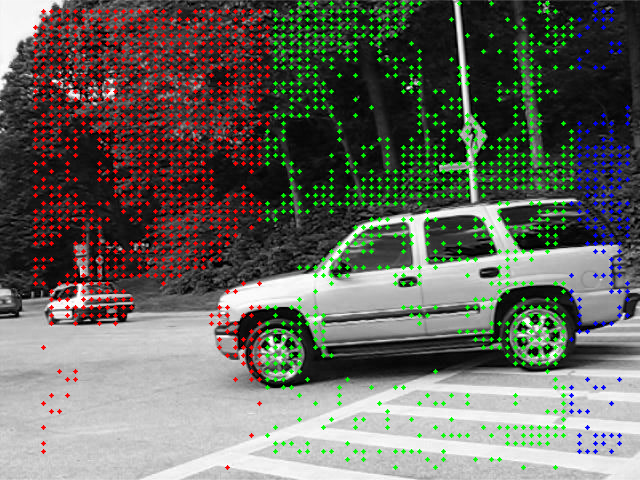
\includegraphics[width=0.175\linewidth] {implementation/mc/0}
   \label{fig:convergence_mc_seg_0}
}
\subfigure[Iteration 1]{
   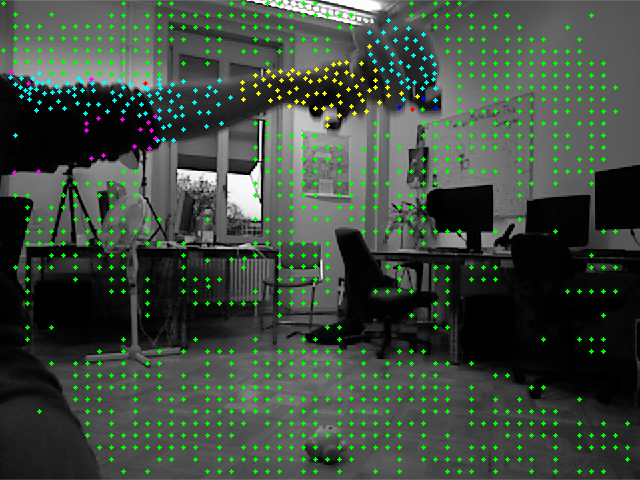
\includegraphics[width=0.175\linewidth] {implementation/mc/1}
   \label{fig:convergence_mc_seg_1}
}
\subfigure[Iteration 2]{
   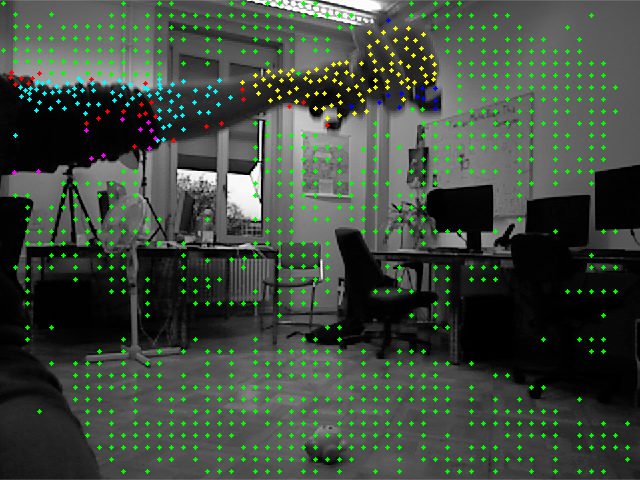
\includegraphics[width=0.175\linewidth] {implementation/mc/2}
   \label{fig:convergence_mc_seg_2}
}
\subfigure[Iteration 3]{
   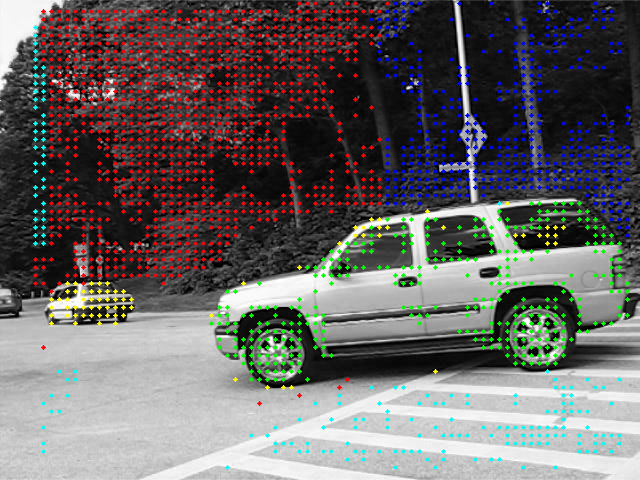
\includegraphics[width=0.175\linewidth] {implementation/mc/3}
   \label{fig:convergence_mc_seg_3}
}
\subfigure[Iteration 4]{
   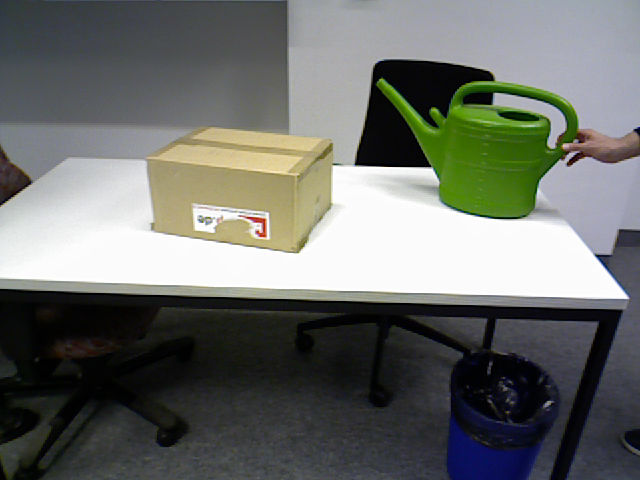
\includegraphics[width=0.175\linewidth] {implementation/mc/4}
   \label{fig:convergence_mc_seg_4}
}
\end{center}
\caption[Convergence MC]{Visualizing the convergence of the MC method (Algorithm $\ref{alg:final_min_cut}$) applied on the Cars$\footnotemark$ dataset when solving for six clusters. The cluster assignments, shown in Figure $\ref{fig:convergence_mc_seg_0}$, are initialized according to Equation $\ref{eq:initialization_min_cut}$. In this example we already observe visual convergence after having run 4 iterations.  }
\label{fig:convergence_mc_seg}
\end{figure} 
\footnotetext{Affinities of the Cars dataset from the BMS-26 dataset from\\ 
\url{http://lmb.informatik.uni-freiburg.de/resources/datasets/}}

\subsection{Kernighan-Lin Heuristic}
\label{sec:kl_impl}
In this section we describe a method that addresses the problem of motion segmentation by formulating it as a minimum cost multi-cut problem on a trajectory similarity graph as defined in Section $\ref{sec:similarity_graphs}$. The energy term \enquote{we optimized to find an optimal graph partition} is based on the work presented in $\cite{KB15b}$. To solve this graph cut problem numerically we implemented the $\textit{Kernighan-Lin}$ heuristic ($\textbf{KL}$) described in $\cite{Ker70}$. \\ \\
In the following, let $G = (E, V)$ denote an undirected graph, where $V$ is the set of vertices and $E$ the set of edges. Moreover, every edge in $E$ has a certain weight $e_c$ assigned. Then, the minimum cost multi-cut problem decomposes the graph $G$ into an optimal number of segments such that the overall edge weights cost is minimized. Equivalently, this vertex labeling problem can be formulated as a binary edge labeling problem, which is defined as
\begin{equation}
\begin{aligned}
& \min_{y \in \{0,1 \}^{|E|}} \sum_{e \in E} c_e y_e \\
& \text{subject to } y \in \text{MC}
\end{aligned}
\end{equation}
The expression $\text{MC}$ denotes the set of characteristic functions of all multi-cuts and thus corresponds to all $y \in \{0,1 \}^{|E|}$ that form closed boundaries. Hence, such boundaries represent a valid decomposition of the graph. To define these characteristics a series of cycle inequalities, similar as done in $\cite{Chopra1993}$, are formulated and defined as follows:
\begin{equation}
	\forall C \in \text{cycles}(G) \forall e \in C: y_e \leq \sum_{e^{'} \in C \backslash \{e\}} y_{e^{'}}
\end{equation}
Furthermore, in $\cite{Chopra1993}$ it was shown, that it is sufficient to only consider those cycles in which each vertex is only connected to its successor and predecessor. \\ \\
In order to avoid trivial solutions when optimizing for these characteristics, we employ the following edge weighting strategy: We chose the weights in such a way that edges, which should be cut, are negative and positive for those which are connected to vertices that should be joined.
In the following, let us assume that we know the edge cut probabilities $p_e$. In that case the negative function
\begin{equation}
	\text{logit}\left( p_e \right) = \log \left( \frac{p_e}{1 - p_e} \right)
	\label{eq:logit_function}
\end{equation}
provides such a desired behavior. A plot of the negative logit function, defined as in Equation $\ref{eq:logit_function}$, is shown in Figure $\ref{fig:negative_logit_function}$.
\begin{figure}[H]
\centering
\begin{tikzpicture}[trim axis left]
\begin{axis}[
  axis x line=center,
  axis y line=center,
  grid=both,
  xtick={-2,-1,...,1,2},
  ytick={-2,-1,...,1,2},
  xlabel={$x$},
  ylabel={$-\text{logit}\left( x \right)$},
  xlabel style={below right},
  ylabel style={above left},
  no markers,
  xmin=-0.5,
  xmax=1.5,
  ymin=-1.5,
  ymax=1.5]
\addplot +[thick, domain=0:1] {-log10(x/(1-x)};
\end{axis}
\end{tikzpicture}
\caption[Logit Function Plot]{A plot of the negative logit function applied on the domain [0,1].}
\label{fig:negative_logit_function}
\end{figure}
If $p_e < 0.5$ then $\text{logit}\left( p_e \right) > 0$ and thus the corresponding edge cost $c_e$ is positive and therefore the edge $e$ is expensive to be cut out from the graph. Conversely, if $p_e > 0.5$ then the negative logit function of $p_e$ is smaller than zero and thus it is beneficial to cut $e$. \\ \\
For computing pseudo-probabilities, we use the inverse of the logit function, the so called \textit{logistic function}
\begin{equation}
	f(z) = \frac{1}{1 + \exp \left( -z \right)}.
	\label{eq:logistic_function}
\end{equation}
This function can therefore be used to define pseudo cut probabilities. Next we have to determine what the input value $z$ represents. Clearly, $z$ is equal to the result of the logit function applied on the pseudo-probability. However, such a definition is not helpful at all, since we defined $f(z)$ as the inverse of the logit and thus end up with a recursive definition. Another interpretation of the negative logit is that it models distances between edges. If the distances are too large, a cut should be performed. Here, the S-affinity distance measure defined in Equation $\ref{eq:sum_dist}$ can be used to compute such a distance $d$. Then, the final expression for $z$ becomes:
\begin{equation}
	z = d - \log \left( \frac{p}{1-p} \right) + \log \left( \frac{\tilde{p}}{1-\tilde{p}} \right).
\label{eq:edge_dist_weights}
\end{equation}
where $p$ is a fixed cut probability and set equals $0.5$ and $\bar{p}$ is a parameter denoting the prior cut probability. If $\bar{p}$ is increased, more edges will be cut and the number of resulting segments increases. Choosing a small $\bar{p}$ results in an undersegmentation. \\ \\
In the following we use discussed formulation to model the similarity graph. In particular we compute its edge weights by using the definition from Equation $\ref{eq:edge_dist_weights}$. Using such negative and positive weights allows us to optimize for the correct number of moving objects including small objects that show discriminative motion in a small number of frames. This approach is supposed to produce more reliable results than the segmentation method described in the section about spectral clustering.
\begin{figure}[H]
\begin{center}
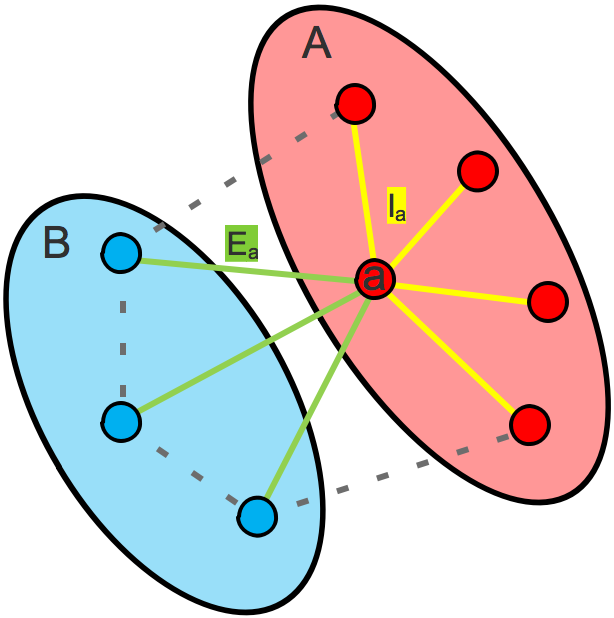
\includegraphics[width=0.6\linewidth] {implementation/segmentation/kl_energies}
\end{center}
\caption[KL Energy Terms]{Visualization of the internal $I_a$ and external costs $E_a$ of a vertex $a \in A$.}
\label{fig:kl_partition_energies}
\end{figure}
Next, let us discuss an algorithm that enables us to partition the similarity graph discussed before. The Kernighan-Lin heuristic $KL$ is a good candidate for this task. This algorithm attempts to find a partition of $V$ into two disjoint subsets $A$ and $B$ of equal size, such that the sum $T$ of edge weights between the vertices in $A$ and $B$ is minimized, similar to Figure $\ref{fig:kl_partition_energies}$. For defining the cost, let $I_a$ be the internal cost of the vertex $a \in A$, which is defined as the sum of the costs of the edges between $a$ and other nodes in $A$. Furthermore, let $E_a$ denote the external cost of $a$, which is defined as the sum of the costs of edges between $a$ and the vertices in $B$. The balance of a vertex is given by the difference defined in Equation $\ref{eq:kl_d_values}$.
\begin{equation}
	D_a = E_a - I_a
\label{eq:kl_d_values}
\end{equation}
If $a$ and $b$ are interchanged, then the reduction in cost is equal to
\begin{equation}
	T_{n} - T_{n-1} = D_a + D_b - 2c_{a,b}
\label{eq:kl_difference_ext_int_costs}
\end{equation}
Note that $c_{a,b}$ in Equation $\ref{eq:kl_difference_ext_int_costs}$ defines the cost of the possible edge between $a$ and $b$. \\ \\
The $KL$ algorithm attempts to find an optimal series of interchange operations between the elements in $A$ and $B$, which maximizes the value of Equation $\ref{eq:kl_difference_ext_int_costs}$. The determined optimal operation sequence is then executed to compute the partition of the graph into the sets $A$ and $B$. \\ \\
In the following we offer the reader some details about the \emph{Kernighan-Lin} heuristic formulated in Algorithm $\ref{alg:kernighan_lin}$. 
\begin{algorithm}[H]
\caption{Kernighan-Lin Algorithm (\textbf{KL2})}
\begin{table}[H]
  \begin{tabular}{@{}lll@{}}
    \textbf{Input:} & Graph \emph{G = (V, E)} \\
    \textbf{Output:} & Binary Graph Partition $\left( A, B \right)$ \\
  \end{tabular} 
\end{table}
\setlength{\fboxrule}{0pt} 
\begin{boxedminipage}{1.0\textwidth}
  \begin{algorithmic}[1]
  	  \State $\text{Determine initial balanced vertex partition into sets A, B}$
      \Do
		\State $\forall a \in A, \forall b \in B: \text{Compute D values}$
		\State $\text{Let gv, av, bv be empty lists}$
		\For{$\text{n=1 to } |V|/2$}
			\State $\text{Find } a \in A, b \in B \text{ such that } g = D_a + D_b - 2e_{a,b} \text{ is maximal}$
			\State $\text{Remove a and b from further consideration in this pass}$
			\State $\text{Put g to gv, a to av, b to bv}$
			\State $\text{Update D values for all elements of } A = A \backslash \{a\}, B = B \backslash \{b\}$
		\EndFor
		\State $\text{Find k that maximizes } g_{max} = \sum_{i=1}^k gv_i$
		\If{$g_{max} > 0$} 
			\State $\text{Exchange } av_1,\dots, av_k \text{ with } bv_1,\dots, bv_k$  
		\EndIf	
      \doWhile{$g_{max} > 0$}
  \end{algorithmic}
  \end{boxedminipage}
  \vskip1.5pt
\label{alg:kernighan_lin}
\end{algorithm}
In this algorithm, we initialize two vertex sets according to some rule. E.g. assign randomly one half of the vertices to set A and the other half to set B. \\ \\
In the inner loop, we determine a ranking of the vertices according to their gain: First, we compute Equation $\ref{eq:kl_d_values}$ on every vertex. Then, we compute the gain between all vertices $a \in A$ and $b \in B$ according to the formulation in Equation $\ref{eq:kl_difference_ext_int_costs}$ and select the vertices $a$ and $b$ that produces the largest gain value. Please note that this can yield negative values. Next, we remember their gain value, mark them as dirty and put each of these vertices into special sets $av$ and $bv$. Afterwards the $D$ values of all vertices, that are not dirty, are updated. We have to repeat this procedure $|V|/2$ times since each set $A$ and $B$ contains that many vertices. \\ \\
In the list of gains we look for the maximal partial sum of gains. The index in the gain list that produced the maximum sum is used as the permutation index for performing a series of interchange operation. Relying on partial sums makes sense, since, as long as the sum increases, the gain in the next iteration gets bigger. We continue permuting until the maximal partial sum would result in having a lower gain in the next outer iteration. We repeat these steps of the most outer loop until there is no more gain. \\ \\
Our Java implementation initially loads the corresponding $\textit{S-affinity}$ matrix and its corresponding nearest neighbor list. Then, an internal undirected graph $G = \left( V, E \right)$ is constructed. Its vertices represent individual trajectories and two vertices are connected if they are actual neighbors. Moreover, The edge weights represent the affinity value between two vertices. Usually, the full neighborhood is loaded into the pipeline and thus the complete graph is formed, i.e. every vertex is interconnected with any other vertex. However, the number of neighbors per trajectory, that should be loaded into the pipeline, can be directly specified by a user via a neighborhood size parameter. \\ \\
An example of the Kernighan-Lin heuristic is illustrated in Figure $\ref{fig:kl_2_part_eg}$.
\begin{figure}[H]
\begin{center}
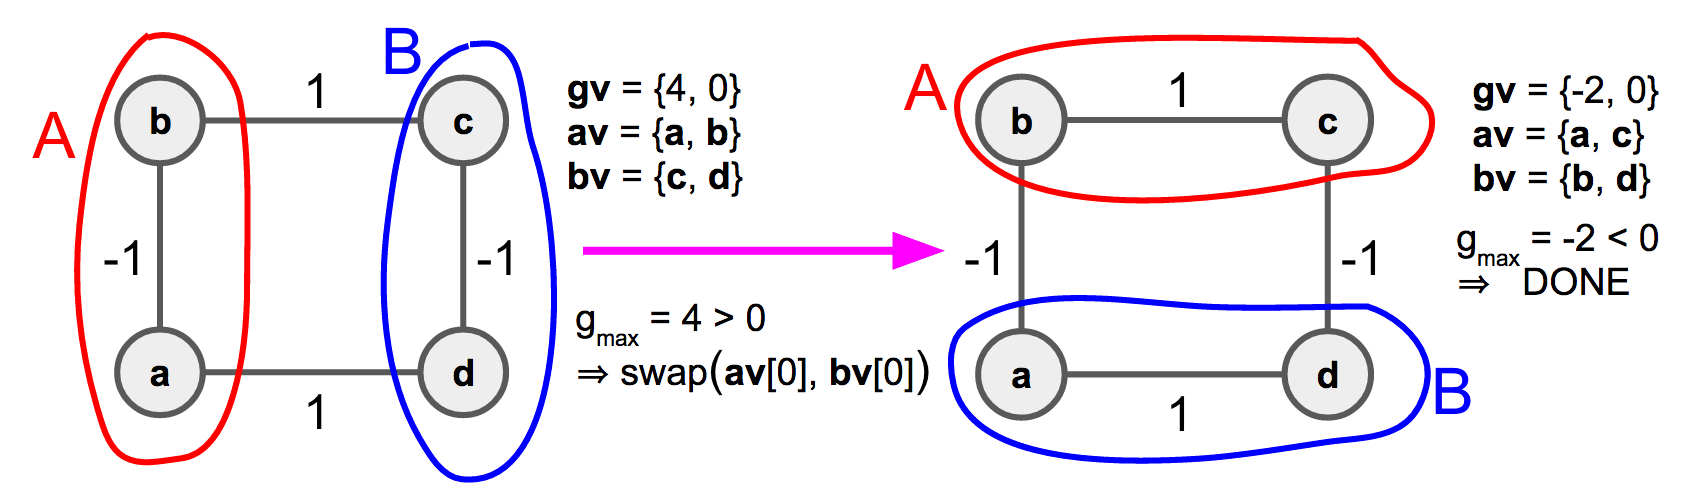
\includegraphics[width=1\linewidth] {implementation/segmentation/kl_2_part_example}
\end{center}
\caption[Kernighan-Lin Example]{An example of Algorithm $\ref{alg:kernighan_lin}$ when solving for two optimal partitions: For two given initial balanced vertex sets $A = \{ a, b\}$ and $B = \{ c, d\}$ (as shown on the left) we want to find the optimal partition of these sets (as shown on the right). Initially, we compute the balance for every vertex according to the definition in Equation $\ref{eq:kl_d_values}$. The corresponding values are listed in the Table $\ref{tab:kl_example_costs}$ (left table). The maximum gain of the first inner loop iteration yields $g_{ac} = 4$ and the second iteration yields $g_{bd} = 0$. Therefore, $g_{max}$ is equal 4 with $k = 1$. Therefore, we have to swap the vertices $a$ and $c$. This will give us the graph partitioning shown on the right. We re-compute the vertex balances and obtain the values shown in the right subtable in Table $\ref{tab:kl_example_costs}$. Since $g_{max}$ is now equal -2, we can stop and have found the optimal graph partitioning $A = \{ b, c\}$ and $B = \{ a, d\}$.}
\label{fig:kl_2_part_eg}
\end{figure}

\begin{table}[H]
\centering
\setlength\tabcolsep{2pt}
\begin{minipage}{0.47\textwidth}
\centering
\begin{tabular}{|c|c|c|c|}
\hline
\multicolumn{4}{|c|}{Initialization} \\ \hline
Vertex $v$ & $I_v$  & $E_v$ & $D_v$ \\ \hline
a & -1 & 1 & 2 \\ \hline
b & -1 & 1 & 2 \\ \hline
c & -1 & 1 & 2 \\ \hline
d & -1 & 1 & 2 \\ \hline
\end{tabular}
\end{minipage}%
\hfill
\begin{minipage}{0.47\textwidth}
\centering
\begin{tabular}{|c|c|c|c|}
\hline
\multicolumn{4}{|c|}{After First Iteration} \\ \hline
Vertex $v$ & $I_v$  & $E_v$ & $D_v$ \\ \hline
a & 1 & -1 & -2 \\ \hline
b & 1 & -1 & -2 \\ \hline
c & 1 & -1 & -2 \\ \hline
d & 1 & -1 & -2 \\ \hline
\end{tabular}
\end{minipage}
\caption[Kernighan-Lin Example Costs]{The internal and external costs and balance values of every vertex of the Kernighan-Lin example, shown in Figure $\ref{fig:kl_2_part_eg}$. On the left the corresponding values after the initialization and on the right the values after the first iteration.}
\label{tab:kl_example_costs}
\end{table}
So far, our KL method is only capable of performing a binary partition on a graph. However, we would like to extend it in such a way, that it can partition a graph into an arbitrary number of labels. \\ \\
To address this problem we apply a greedy strategy. Let us assume that we want to solve for $k$ clusters and we are working with $n$ vertices. Then, we distribute the $n$ vertices according to some initialization rule among $k$ empty sets. Then, for each possible pair of subsets we sequentially run Algorithm $\ref{alg:kernighan_lin}$, which gives us the pairwise optima. We repeat this procedure until the solution has converged. Our final $KL$ algorithm that we use to solve the multi-cut problem is listed in Algorithm $\ref{alg:kl_multiple_segments}$.
\begin{algorithm}[H]
\caption{Kernighan-Lin Multicut Heuristic (\textbf{KL})}
\begin{table}[H]
  \begin{tabular}{@{}lll@{}}
    \textbf{Input:} & Graph \emph{G = (V, E)} \\
        & Number of segments C \\
    & Number of repetitions N  \\
    & Number of dummy vertices D \\
	\textbf{Output:} & Multiple Graph Partition $\left( A_1,\dots, A_N \right)$ 
  \end{tabular} 
\end{table}
\textbf{Procedures:} $KernighanLin(G)$  \\
\setlength{\fboxrule}{0pt} 
\begin{boxedminipage}{1.0\textwidth}
  \begin{algorithmic}[1]
  	\For{$n = 1 : N$}
  	  \State $\text{Split V into C initial balanced sets} A_1,\dots,A_C$
  	  \State $\text{Append D dummy vertices to each initial set} A_k$ 
      \ForAll{$\text{distinct vertex set pair} \left( A_k, A_l\right)$}
        \State $ \text{Form the subgraph } G_{k,l} = (V, E)$
		\State $\text{Run the two partition Kernighan-Lin Algorithm } KL2(G_{k,l}) \text{ and Update G}$
      \EndFor
    \EndFor{$\text{d}$}
  \end{algorithmic}
  \end{boxedminipage}
  \vskip1.5pt
\label{alg:kl_multiple_segments}
\end{algorithm}
In our implementation we want to use the following initialization: One set among the $k$ sets is initialized with all $n$ vertices and the other sets are empty. This will give every set the same change to get some vertices in a fair amount of time. However, this also violates our restriction that \textit{the subsets have to be of equal size}. The solution to this problem is to introduce so-called \textit{dummy vertices}, which are placeholders and exhibit zero similarities. This means that they do not affect the cost terms used during the optimization. Additionally, Figure $\ref{fig:kl_multipart_label}$ visualizes one iteration of Algorithm $\ref{alg:kl_multiple_segments}$.
\begin{figure}[H]
\begin{center}
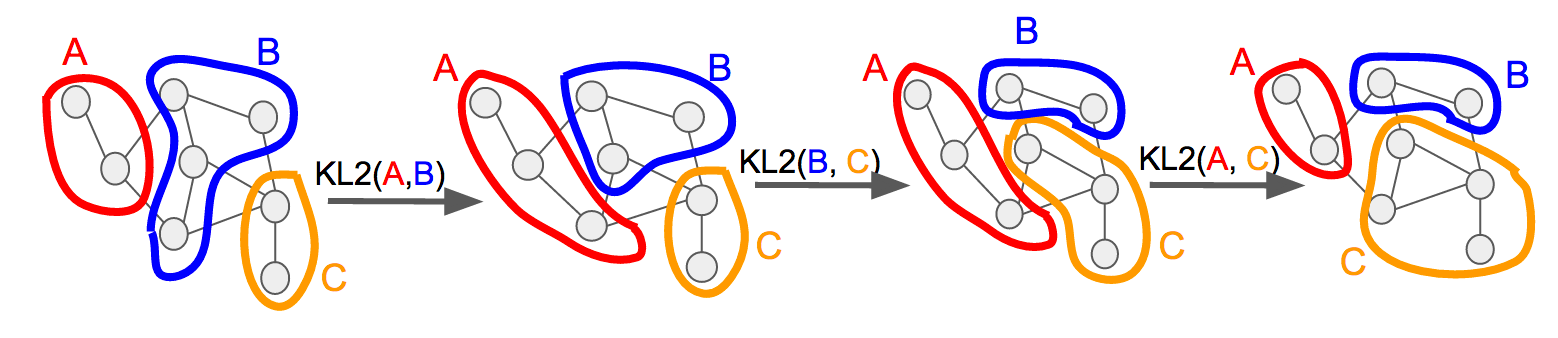
\includegraphics[width=1\linewidth] {implementation/segmentation/kl_multiple_clusters_example}
\end{center}
\caption[Kernighan-Lin 3 Partitions Example]{In this example we show one iteration of Algorithm $\ref{alg:kl_multiple_segments}$ when solving for three optimal partitions on a given graph. We initially partition our graph into three optimal partitions $A$, $B$, $C$ as shown on the left image. Set A and set B contain dummy vertices. Then, we run the Kernighan-Lin \textbf{KL2} (Algorithm $\ref{alg:kernighan_lin}$) on every possible set pair and update the graph accordingly. The final result after one iteration is shown on the right.}. 
\label{fig:kl_multipart_label}
\end{figure}

\section{Dense Motion Segmentation}
\label{sec:dense_motion_segmentation}
From this moment on we are able to generate sparse motion segmentations by using three different methods: Spectral Clustering \textit{SC} (Sec. $\ref{sec:spectral_clustering_impl}$), Minimum Cut\textit{MC} (Sec. $\ref{sec:min_cut_seg}$) and Kernighan-Lin \textit{KL} (Sec. $\ref{sec:kl_impl}$). However, in some vision related tasks, it would make sense to determine dense masks. This would enable us to extract moving objects by simply applying the corresponding mask. However, keep in mind that generating dense motion segmentations is not the focus of this \enquote{work} and therefore will not be evaluated. \\ \\
In this section we describe a simple method to produce a dense motion segmentations from previously generated sparse segmentations. For this purpose we adapted an existing implementation, which addresses the problem of demosaicing an image by formulating it as a convex optimization problem. The problem is reformulated in its primal-dual form and an iterative solver was developed. A detailed derivation can be found in the appendix in Chapter $\ref{chap:appendix_demosaicing}$. I developed this program during a semester project in the class \textit{Convex Optimization} in 2015 held by Prof. Dr. P. Favaro at the University of Bern. The class was based about the book Convex Optimization by Boyd and Vanderberg $\cite{BoydVanderberg2004}$. The class, as well as the implementation and the derivation assume a certain knowledge in convex problem formulations and how to solve such problems. \\ \\
The idea is to interpret the sparse segmentation as an image with missing data due to its sparsity. Therefore, we aim to solve the problem of hole filling, which is the same as finding the demosaiced image by using our formulation. \\ \\
For a given image with missing data $g$ we want to find its reconstructed image $u$. This can be achieved by minimizing an energy term $E$ which is defined as 
\begin{equation}
	E(u) = \underbrace{\norm{\nabla u}_2}_{\text{smoothness term}} + \frac{\lambda}{2} \underbrace{\norm{u - g}^2_{\Omega}}_{\text{data term}}	
\end{equation}
where we defined its data term as
\begin{equation}
\begin{aligned}
& \norm{u - g}^2_{\Omega_{C}} = \sum_x \sum_y \Omega_{C}(x,y)\norm{u(x,y) - g(x,y)}^2 \\
& \text{where } \Omega_{C}(x,y)= 
\begin{cases}
    0,& \text{if } $g(x,y)$ \text{ is missing}\\
    1,              & \text{otherwise}
\end{cases}
\end{aligned}
\end{equation}
First let us have a look at the \textbf{data term}. It ensures that the reconstructed image does not deviate too much from the given input $g$ w.r.t the norm $\norm{\cdot}_\Omega$. This norm only operates on image locations that exhibit existing pixel data. Therefore, we have to skip every invalid image location in $g$, when applying this norm on the difference between $u$ and $g$. The \textbf{smoothness term} ensures a smooth transition between the colors in the image.
\begin{figure}[H]
\begin{center}
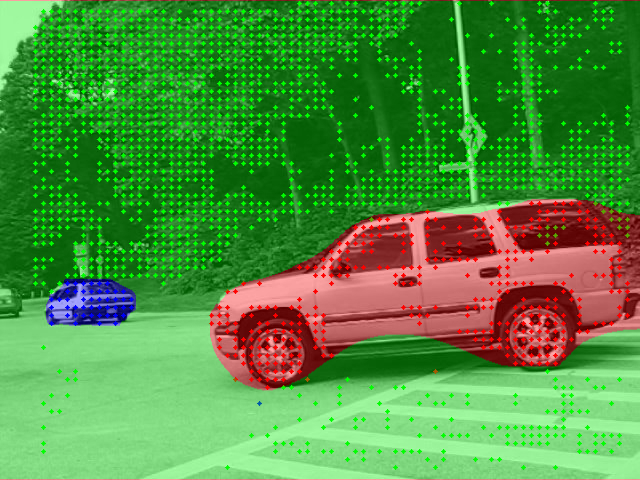
\includegraphics[width=0.8\linewidth] {implementation/dense_seg/cars_1}
\end{center}
\caption[Dense Segmentation Cars]{A dense segmentation$\footnotemark$ produced by our pipeline. We see an overlay of the sparse segmentation on top of the dense masks. As we can see, the dense segmentation is basically a blur of the initial given sparse segments.}
\label{fig:dense_segmentation_cars_1}
\end{figure}
\footnotetext{To generate Figure $\ref{fig:dense_segmentation_cars_1}$ I used the Cars dataset from the BMS-26 dataset: Source\\ 
\url{http://lmb.informatik.uni-freiburg.de/resources/datasets/}}
In Section $\ref{sec:primal_dual_form}$ described how to solve this optimization problem by formulating its Primal-Dual form. Such a formulation allows us to derive an iterative solver to address this optimization. A detailed, step by step derivation can be found in the appendix in Chapter $\ref{chap:appendix_demosaicing}$. One iteration of our solver runs the following steps:
\begin{equation}
\begin{aligned}
	y^{n+1} &= \frac{y^n + \sigma \nabla \bar{x}^{n}}{\max{\left(1,\twonorm{y^n + \sigma \nabla \bar{x}^{n}} \right)}} \nonumber \\
	x^{n+1} &= \frac{x^n - \tau \left[ \left( \partial_x y_{x}^{n+1} + \partial_y y_{x}^{n+1} \right) + \left( \partial_x y_{y}^{n+1} + \partial_y y_{y}^{n+1} \right) \right] +  \tau \lambda \Omega g}{1+\tau \lambda \Omega} \\
	\bar{x}^{n+1} &= x^{n+1} + \theta(x^{n+1} - x^n)
\end{aligned}
\end{equation}
Here, $x^n$ (Sec. $\ref{sec:pd_xn}$) and $y^n$ (Sec. $\ref{sec:pd_yn}$) denote the Primal-Dual steps of our optimization problem and $\bar{x}^n$ denotes a gradient descend step used to approach a local optimum of our dense segmentation. For computing $\nabla$ we rely on a forward difference approximation scheme. We repeat this update rule until $\norm{\bar{x}^{n+1} - \bar{x}^{n}}$ is small enough. Moreover, we use the parameter assignment listed in Equation $\ref{eq:parameter_set_up}$. \\ \\
A dense segmentation, produced by running this method, is shown in Figure $\ref{fig:dense_segmentation_cars_1}$. This figure shows the dense segments as colored masks. Additionally, we also show the sparse segmentation, using the same colors. As we can see, the dense segmentation is basically a blurred version of the initial sparse input. 